\chapter{การออกแบบและวิธีการดำเนินงาน}

%%%%%%%%%%%%%%%%%%%%%%%%%%%%%%%%%%%%%%%%%%%%%%%%%%%%%%%%%%%%%
% User Survey Section
%%%%%%%%%%%%%%%%%%%%%%%%%%%%%%%%%%%%%%%%%%%%%%%%%%%%%%%%%%%%%

\section{การสำรวจความต้องการกับผู้ใช้}
ทางคณะผู้จัดทำได้ทำออกเก็บข้อมูลกับกลุ่มเป้าหมายมาแล้วทั้งหมด 4 ครั้ง โดยแบ่งเป็นการสัมภาษณ์เชิงปริมาณหนึ่งครั้งและเชิงคุณภาพสามครั้ง  โดยมีจุดประสงค์ในแต่ละการสัมภาษณ์ต่างกันเพื่อพิสูจน์ความต้องการของกลุ่มเป้าหมายจนกระทั่งโครงงานของเราได้ปรับตามความต้องการนั้นจนเป็นโครงงานในปัจจุบัน อย่างไรก็ตาม เรายังได้รับข้อมูลที่น่าสนใจเพิ่มเติมโดยสรุป ดังนี้

\subsection{การสัมภาษณ์เชิงปริมาณผ่านแบบสำรวจ}
ทางคณะผู้จัดทำได้ทำแบบสอบถามเพื่อหาอัตราส่วนของพฤติกรรมที่น่าสนใจ โดยได้รับข้อมูลที่สำน่าสนใจดังนี้
\begin{figure}[!h]\centering
    \setlength{\fboxrule}{0.2mm} % can define this in the preamble
    \setlength{\fboxsep}{0.5cm}
    \fbox{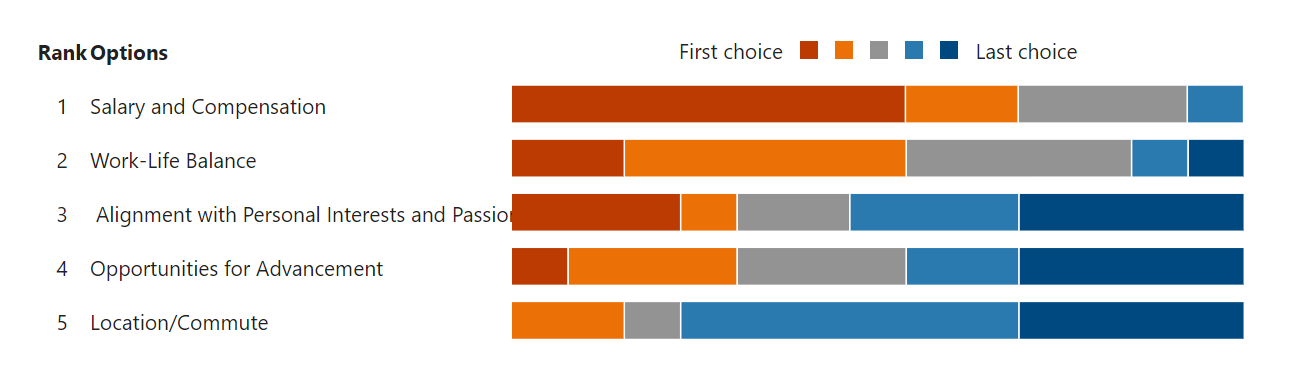
\includegraphics[width=10cm]{./figure/figure_poll.png}}
    \caption{ข้อมูลจากแบบสำรวจเชิงปริมาณ}\label{fig:insightPoll}
\end{figure}
จากข้อมูลในแบบสำรวจข้อนี้ ทำให้ทราบว่าปัจจัยที่มีผลต่อการเลือกสายงานในการทำงานมากสำหรับกลุ่มตัวอย่างก็คือเงินเดือน และความสมดุลของการทำงานกับชีวิตส่วนตัว กล่าวคือกลุ่มตัวอย่างให้ความสำคัญกับความจริงมากยิ่งขึ้น ความมั่นคง หรือเงินเดือนที่สามารถทำให้ดำเนินชีวิตได้อย่างราบรื่น รวมถึงการแบ่งเวลา การพักผ่อนที่เหมาะสมกับการทำงาน โดยมองอาจจะไม่ได้ให้ความสำคัญกับความชื่นชอบมากขนาดนั้น

\subsection{การสัมภาษณ์เชิงคุณภาพผ่านการสัมภาษณ์ตัวต่อตัว}
ทางคณะผู้จัดทำได้ออกสัมภาษณ์กับกลุ่มเป้าหมายแบบตัวต่อตัว และในการสัมภาษณ์แต่ละครั้ง จะสัมภาษณ์ที่จำนวน 5 คน ตามหลักการ 5 Users design โดยได้รับข้อมูลที่น่าสนใจในแต่ละครั้งมาดังนี้
\newline
\textbf{การสัมภาษณ์เชิงคุณภาพครั้งที่ 1}
\newline
\textbf{จุดประสงค์: เพื่อค้นหารากขอปัญหาที่แท้จริงของกลุ่มเป้าหมาย}
\newline
\textbf{ข้อมูลสำคัญ: }
\begin{itemize}
    \item กลุ่มเป้าหมายค้นพบความต้องการของตนเองมาจากการได้ลงมือทำจริงเป็นหลัก
    \item ส่วนใหญ่แล้วจะได้ลงมือทำจริงตอนโปรเจ็กต์วิชาเรียนหรือฝึกงาน ซึ่งอยู่ชั้นปีที่ 2 เป็นต้นไปแล้ว
    \item อยากรู้ก่อนเป็นอย่างมาก ว่าในการทำงานจริงต้องมีความสามารถอะไรบ้าง ใช้เครื่องมืออะไร
    \item กลุ่มเป้าหมายรู้สึกว่าอาจรู้ตัวช้าเกินไป หากมีโอกาสพัฒนาตนเองได้เร็วกว่านี้จะดีมาก
\end{itemize}


\noindent\textbf{การสัมภาษณ์เชิงคุณภาพครั้งที่ 2}
\newline
\textbf{จุดประสงค์: เพื่อพิสูจน์ความมีคุณภาพของวิธีการแก้ปัญหาที่ออกแบบ}
\newline
\textbf{ข้อมูลสำคัญ: }
\begin{itemize}
    \item กลุ่มเป้าหมายอยากได้ตัวช่วยในการทำให้ตนเองสมัครงานได้ง่ายขึ้น โดยหลังการทดลองถามความเห็น พบว่าสิ่งที่ต้องการเป็นหลักคือ การตรวจสอบและยืนยันได้ ว่าเรซูเม่ของตนเองเหมาะสมกับอาชีพที่ตนเองสนใจขนาดไหนแล้ว
    \item กลุ่มเป้าหมายรู้สึกสนใจในฟีเจอร์ช่วยเหลือการค้นหาแหล่งพัฒนาตนเอง เพราะเคยรู้สึกว่าตนเองอาจเริ่มพัฒนาช้าเกินไป เพราะรู้ใจตัวเองในช่วงที่อาจเรียนอยู่ชั้นปีที่ 2-3 แล้ว
    \item การตัดสินใจลงวิชาเรียนค่อนข้างมีจุดขัดใจ เพราะไม่ค่อยมีรีวิวหรือความเห็นของผู้ที่เคยเรียน ถึงแม้เคยมีแหล่งชุมชนที่รุ่นพี่เคยมอบให้ แต่รีวิวส่วนใหญ่จะมีความเก่าแล้ว ทำให้ใช้อ้างอิงได้ยาก
\end{itemize}


\noindent\textbf{การสัมภาษณ์เชิงคุณภาพครั้งที่ 3}
\newline
\textbf{จุดประสงค์: เพื่อทดลองนำ prototype ของเว็บแอปไปพิสูจน์ความรู้สึกในการใช้งานกับผู้ใช้}
\newline
\textbf{ข้อมูลสำคัญ:}
\begin{itemize}
    \item ผู้ใช้ไม่มีปัญหากับการกรอกข้อมูลเรซูเมเพื่อวิเคราะห์ แต่หากมีระบบที่กรอกข้อมูลให้อัตโนมัติผ่านไฟล์ pdf ก็ถือว่าเป็นเรื่องดี
    \item การมีระบบโหวตวิชาที่อยากให้เปิด อาจไม่ได้เป็นการการันตีว่าจะเปิดได้จริง อาจไม่สำคัญมากนัก
    \item ในอนาคต หากมีระบบที่เป็นตัวช่วยในการสร้างเรซูเมจากข้อมูลที่มีได้ ก็จะเป็นเรื่องที่ดีเช่นกัน
    \item ควรมีการแบ่ง tag ประเภทของชุมชนเพื่อความสะดวกในการค้นหา
\end{itemize}

%%%%%%%%%%%%%%%%%%%%%%%%%%%%%%%%%%%%%%%%%%%%%%%%%%%%%%%%%%%%%
% System Functional Section
%%%%%%%%%%%%%%%%%%%%%%%%%%%%%%%%%%%%%%%%%%%%%%%%%%%%%%%%%%%%%

\section{ความสามารถของระบบ}
\subsection{Use Case Diagram}
\begin{figure}[H]\centering
    \setlength{\fboxrule}{0.2mm} % can define this in the preamble
    \setlength{\fboxsep}{0.5cm}
    \fbox{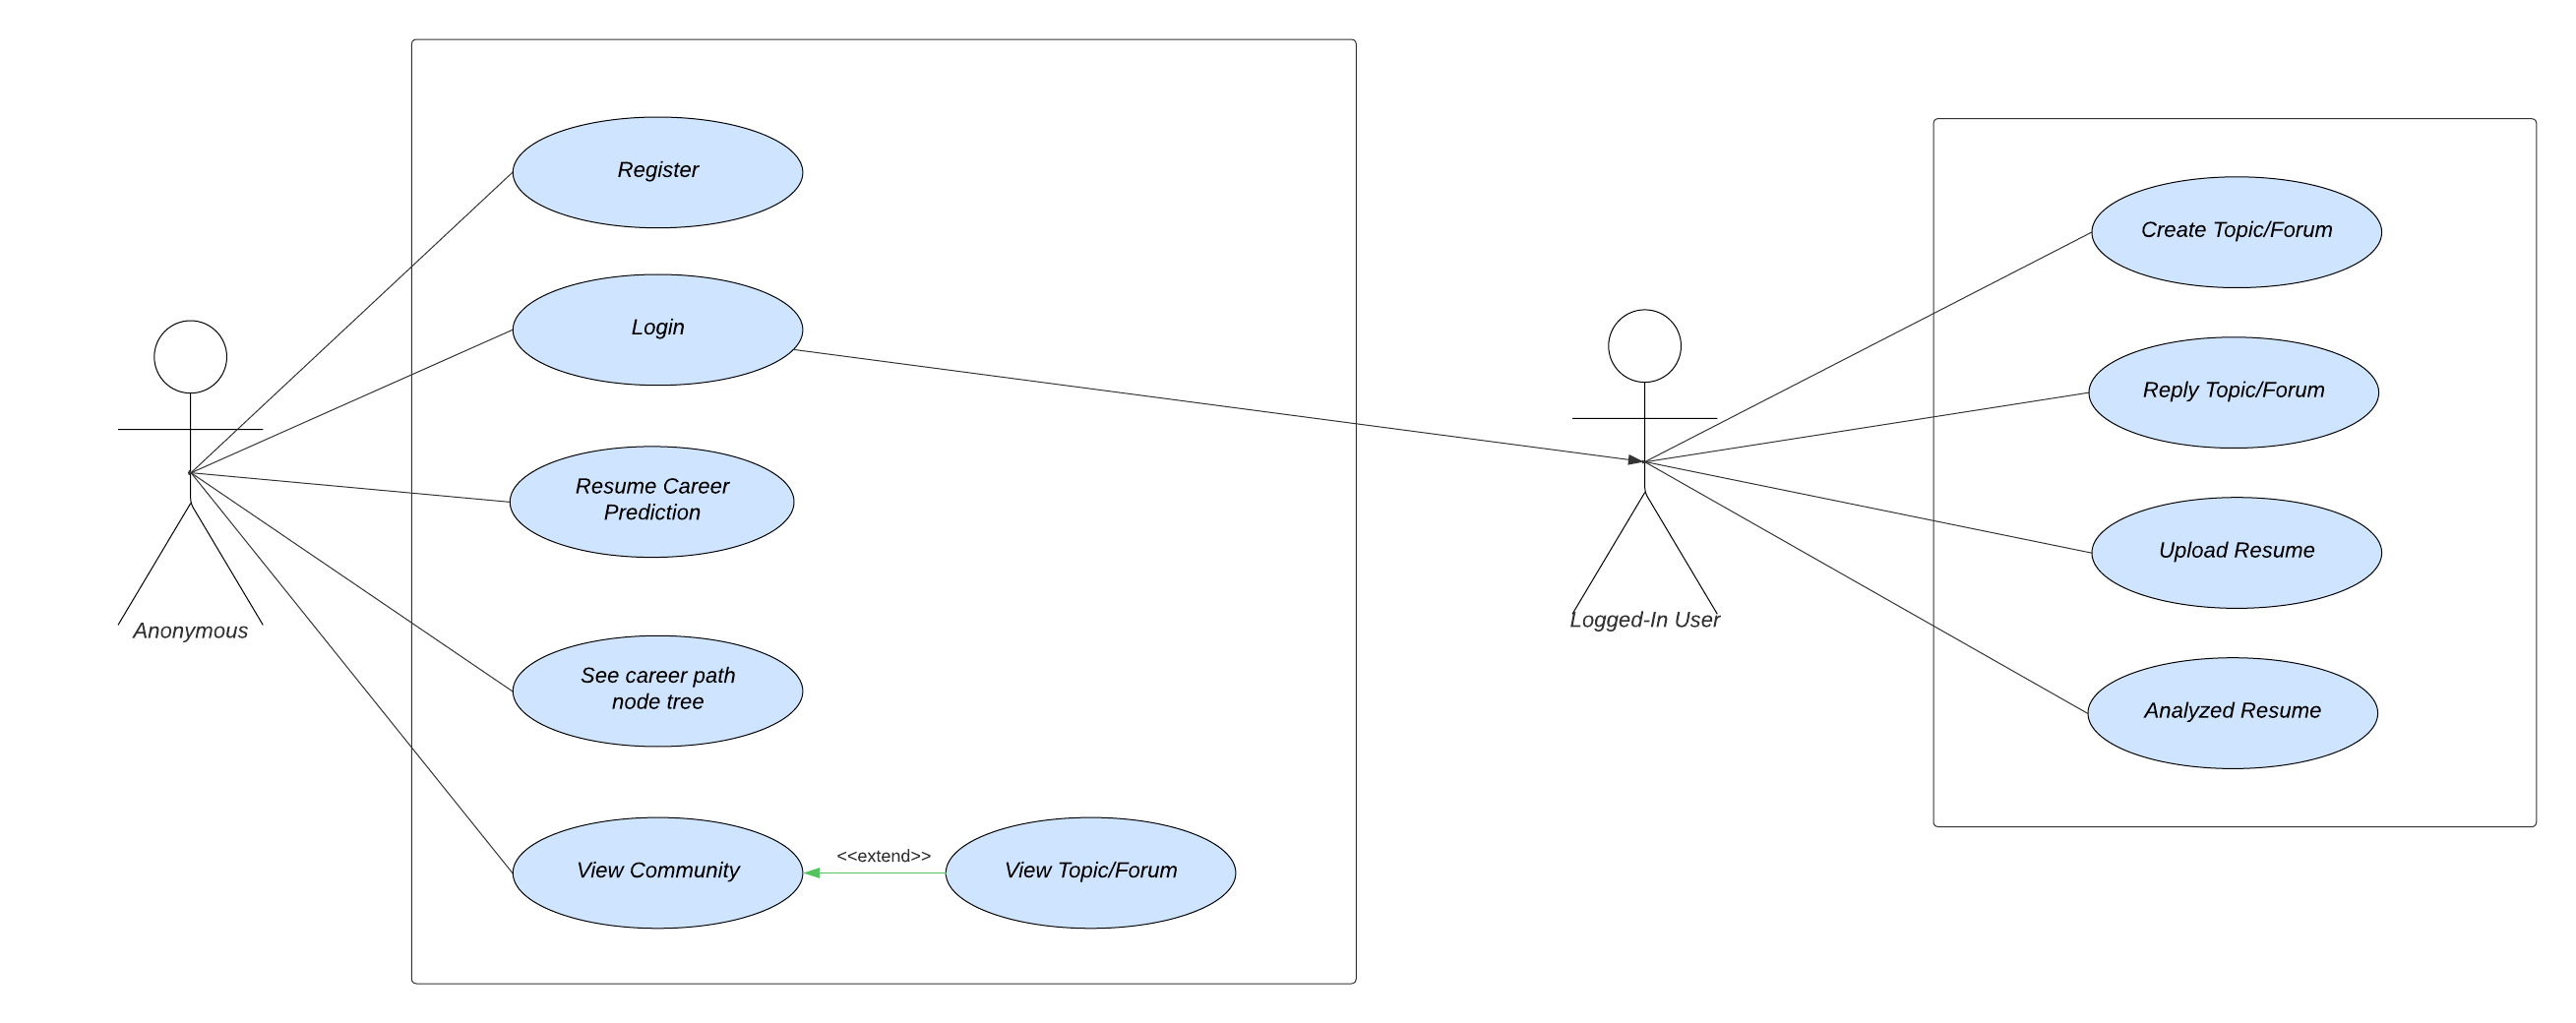
\includegraphics[width=10cm]{./figure/figure_usecase.png}}
    \caption{Use Case Diagram}\label{fig:usecase}
\end{figure}
\subsection{Use Case Narrative}
\subsubsection{Resume Career Prediction}
\begin{table}[H]
    % \centering
    \begin{tabularx}{\textwidth}{|l|X|} 
        \hline
        Actor                 & User                                       \\ \hline
        Goal                  & ต้องการทราบถึงอาชีพที่เหมาะสมกับตนเองจากข้อมูลในเรซูเม            \\ \hline
        Precondition          & -                                               \\ \hline
        Main success scenario & 1. ผู้ใช้กดปุ่มทำนายผล                         \\
        & 2. ระบบถามข้อมูลของผู้ใช้                            \\
        & 3. ผู้ใช้กรอกข้อมูลเรซูเม                                  \\
        & 4. ผู้ใช้กดปุ่มทำนายผล                                \\
        & 5. ระบบตรวจสอบข้อมูลที่ผู้ใช้กรอก                           \\
        & 6. ระบบแสดงอาชีพที่เหมาะสมกับผู้ใช้                    \\
        & 7. บันทึกประวัติการทำนายผลลงในระบบ           \\ \hline
        Extensions (a)        & 5a. ผู้ใช้กรอกข้อมูลไม่ครบ                            \\
        & 6a. ระบบขึ้นเตือนว่าผู้ใช้ยังกรอกข้อมูลไม่ครบ              \\
        & 7a. กลับไปที่ขั้นตอนที่ 3                              \\ \hline
        Postcodition          & ระบบแนะนำให้ผู้ใช้ไปวิเคราะห์ข้อมูลเชิงลึกของอาชีพที่ได้แนะนำไป \\ \hline
    \end{tabularx}
\end{table}

\subsubsection{Watch Career Insight}
\begin{table}[H]
    % \centering
    \begin{tabularx}{\textwidth}{|l|X|} \hline
        Actor                 & User                  \\ \hline
        Goal                  & ต้องการดูข้อมูลเชิงลึกของอาชีพ         \\ \hline
        Precondition          & ผู้ใช้ต้องมีอาชีพที่ระบบแนะนำให้ในประวัติ          \\ \hline
        Main success scenario & 1. ผู้ใช้เลือกอาชีพที่ต้องการดูข้อมูลเชิงลึก \\
        & 2. ระบบแสดงข้อมูลเชิงลึกของอาชีพ     \\ \hline
        Extensions (a)        & 1a. ผู้ใช้ต้องวิเคราะห์อาชีพใหม่        \\
        & 2a. ระบบถามถึงข้อมูลของผู้ใช้         \\
        & 3a. ผู้ใช้กรอกข้อมูลใหม่              \\
        & 4a. ผู้ใช้ยืนยันการกรอกข้อมูล          \\
        & 5a. ระบบแสดงอาชีพที่เหมาะสมกับผู้ใช้   \\
        & 6a. กลับไปที่ขั้นตอนที่ 1              \\ \hline
        Postcodition          & -                               \\ \hline
    \end{tabularx}
\end{table}


%%%%%%%%%%%%%%%%%%%%%%%%%%%%%%%%%%%%%%%%%%%%%%%%%%%%%%%%%%%%%
% System Architecture Section
%%%%%%%%%%%%%%%%%%%%%%%%%%%%%%%%%%%%%%%%%%%%%%%%%%%%%%%%%%%%%

\section{สถาปัตยกรรมของระบบ}
\begin{figure}[H]\centering
    \setlength{\fboxrule}{0.2mm} % can define this in the preamble
    \setlength{\fboxsep}{0.5cm}
    \fbox{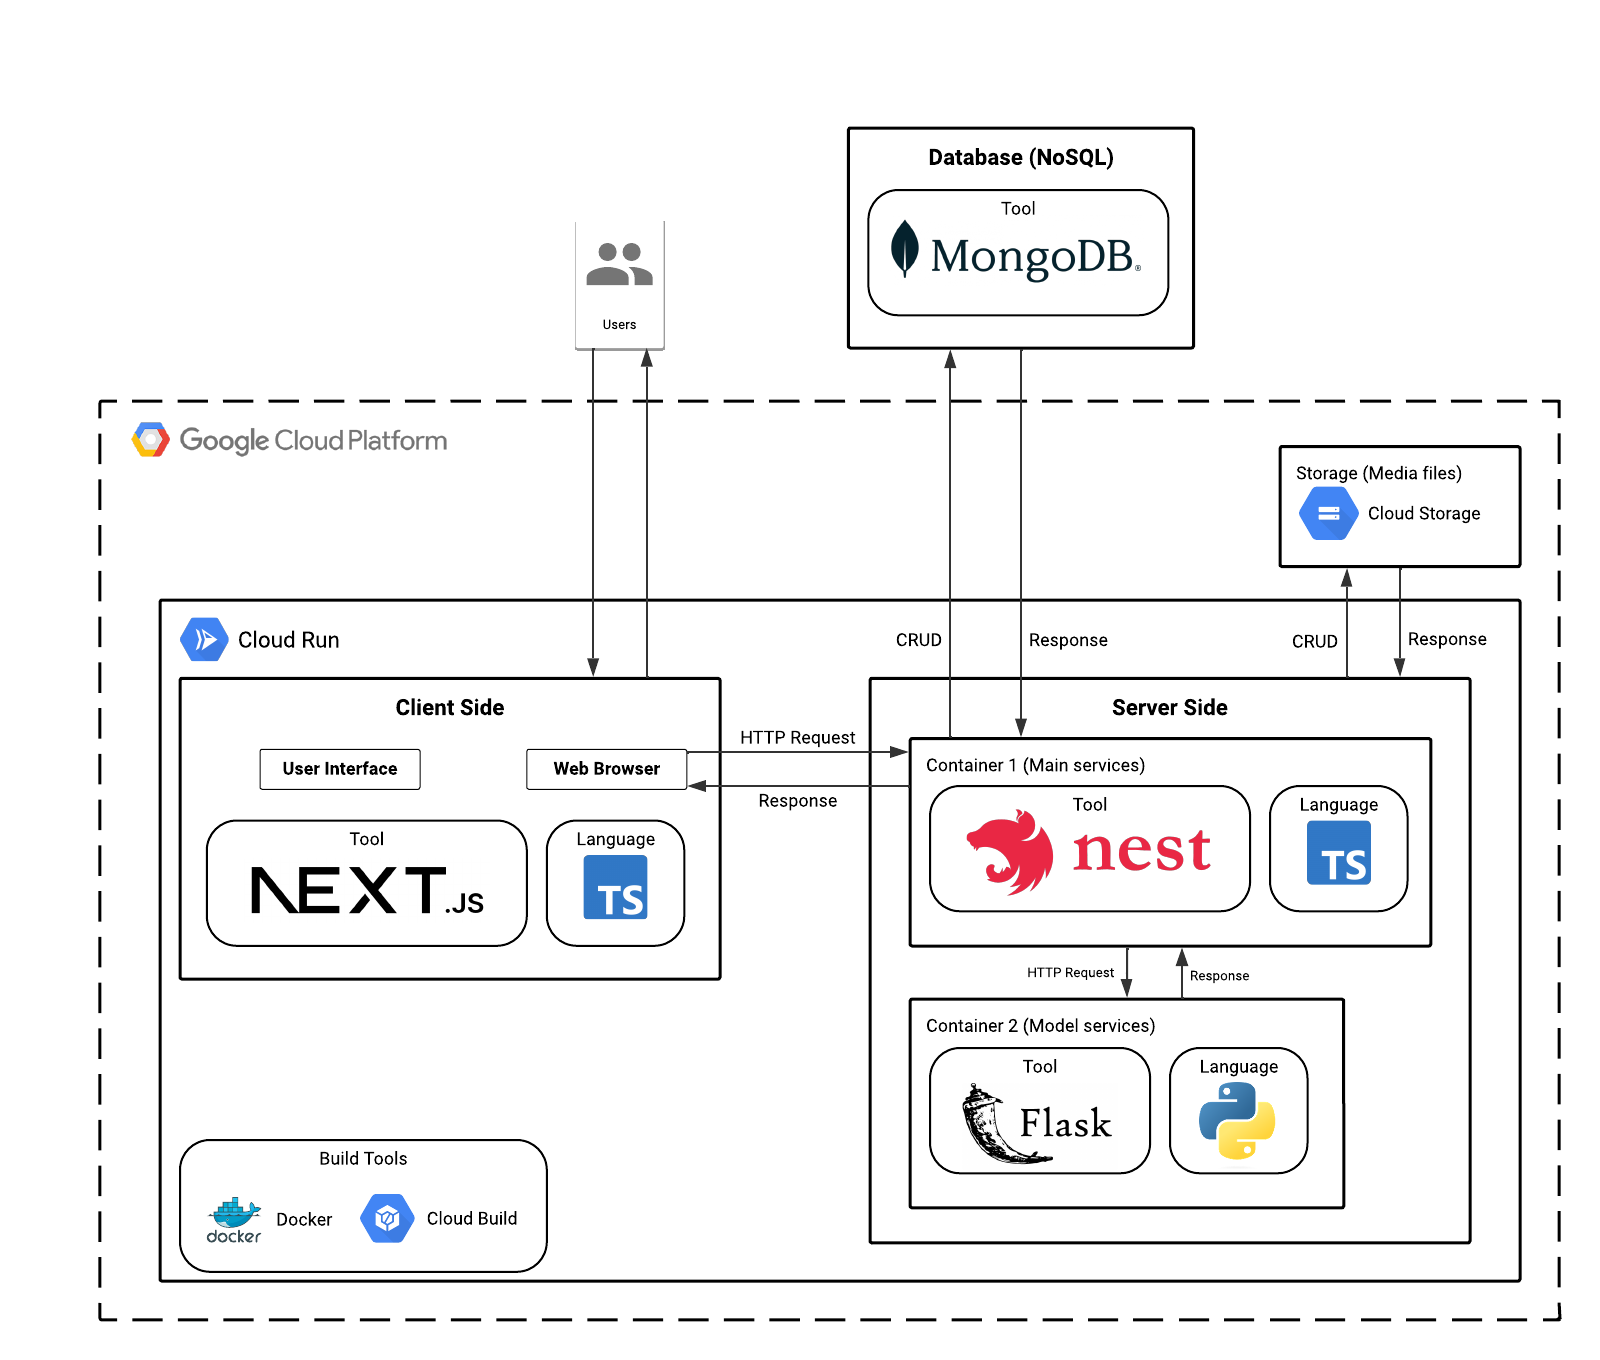
\includegraphics[width=10cm]{./figure/figure_system_architecture.png}}
    \caption{System Architecture}\label{fig:system_architecture}
\end{figure}
จากแผนผังสถาปัตยกรรมระบบ เราได้ใช้บริการ Google Cloud เป็นหลักเนื่องจากสะดวกต่อการ scaling ในอนาคต สามารถจัดการและเปลี่ยนแปลงเวอร์ชันได้รวดเร็วระหว่างการพัฒนา โดยสถาปัตยกรรมแต่ละส่วนมีหน้าที่หลักดังนี้

\subsection{ส่วนผู้ใช้ (Client-Side)}
รับผิดชอบในการติดต่อปฏิสัมพันธ์กับผู้ใช้ แสดง user interface ผ่านทาง web browser และเชื่อมต่อกับ server เพื่อขอข้อมูลและใช้บริการต่าง ๆ

\subsection{ส่วนเซิร์ฟเวอร์ (Server-Side)}
รับผิดชอบในการจัดการตรรกะและระบบคำนวณต่าง ๆ ทุกรูปแบบและส่งกลับไปให้ผู้ใช้ โดยทางคณะู้จัดทำได้แบ่งระบบ server เป็นสองบริการหลัก ประกอบด้วย
\newline
1. บริการหลัก (Main services)
\newline
บริการที่จะติดต่อกับผู้ใช้โดยตรงเพียงหนึ่งเดียว มีหน้าที่ในการจัดการทุกคำขอจากผู้ใช้ผ่านทาง API (Application Programming Interfaces) เช่น ดึงข้อมูลจากฐานข้อมูล คำนวณค่าต่าง ๆ และติดต่อกับบริการอื่น ๆ
\newline
2. บริการโมเดล (Model services)
\newline
บริการสำหรับใช้คำนวณเกี่ยวกับปัญญาประดิษฐ์ของทางคณะผู้จัดทำเท่านั้น เนื่องจากกินทรัพยากรสูง การแยกบริการออกมาจากบริการหลักจึงสามารถดูแลและจัดการได้ง่ายกว่า โดยจะรับค่ามาจากส่วนบริการหลักและส่งค่ากลับไปให้


\subsection{Architecture Pattern}
\begin{figure}[H]\centering
    \setlength{\fboxrule}{0.2mm} % can define this in the preamble
    \setlength{\fboxsep}{0.5cm}
    \fbox{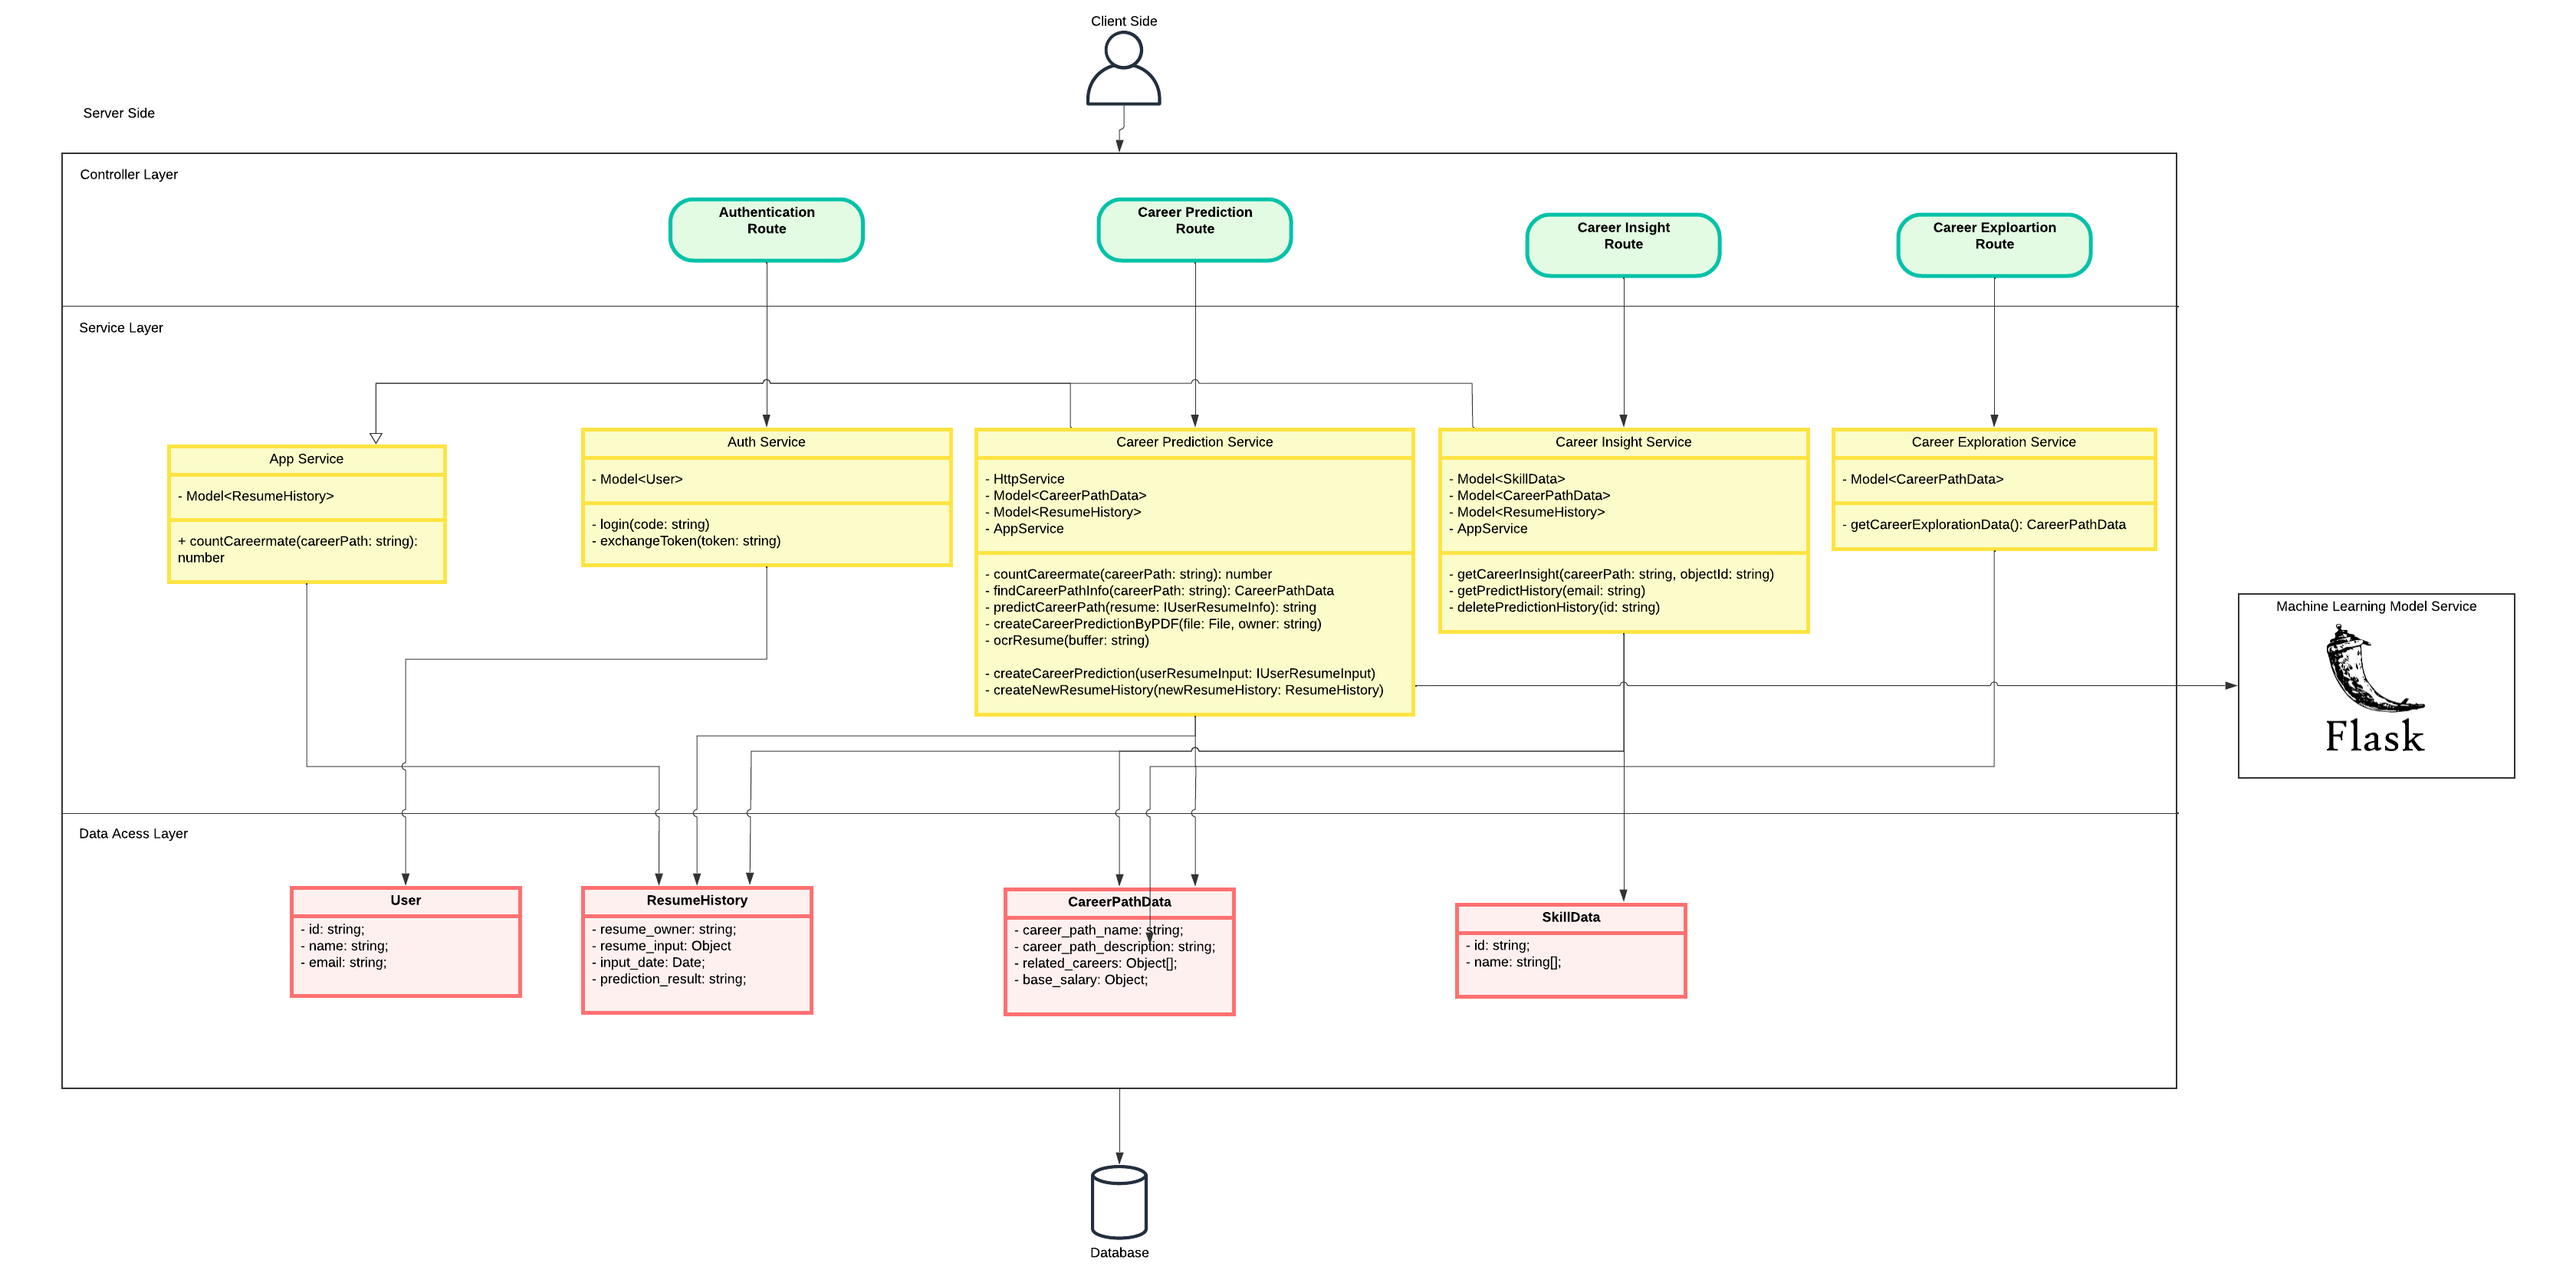
\includegraphics[width=8cm]{./figure/figure_architecture_pattern.png}}
    \caption{Architecture Pattern}\label{fig:arch_pattern}
\end{figure}
เพื่อการพัฒนาซอฟต์แวร์ร่วมกันที่มีประสิทธิภาพ และการจำแนกหน่วยการทำงานของระบบได้อย่างชัดเจน เราจึงได้ออกแบบ Architecture Pattern ตามหลักการของ NestJs ซึ่งประกอบด้วย 3 ระดับคือ

\begin{enumerate}
    \item Route รับหน้าที่ในการรับมือทางเข้าที่ผู้ใช้สามารถส่งคำขอทั้งหมดมาที่ระบบหลังบ้าน และเรียกใช้งานบริการภายใน เช่น การขอยืนยันตัวตน การขอเข้าชมข้อมูลเชิงลึก เป็นต้น
    \item Service หน่วยบริการที่รับหน้าที่ดำเนินการเชิงตรรกะและคำนวณทั้งหมดตามหมดหมู่ เพื่อส่งกลับข้อมูลไปที่ผู้ใช้ หรือเรียกใช้ข้อมูลจากฐานข้อมูลผ่าน Data Acess เช่น บริการยืนยันตัวตน เพื่อรับหน้าที่ยืนยันตัวตน สร้างและส่งโทเคนกลับสู่ผู้ใช้
    \item Data Access เป็นส่วนเชื่อมต่อกับฐานข้อมูลตามแผนภาพข้อมูลที่ประกาศไว้ ถูกแบ่งไว้ตามหมวดหมู่ตาม collection ในฐานข้อมูล และส่งกลับข้อมูลที่ตรงกันกลับสู่หน่วยบริการ
\end{enumerate}


%%%%%%%%%%%%%%%%%%%%%%%%%%%%%%%%%%%%%%%%%%%%%%%%%%%%%%%%%%%%%
% Sequence Diagram Section
%%%%%%%%%%%%%%%%%%%%%%%%%%%%%%%%%%%%%%%%%%%%%%%%%%%%%%%%%%%%%

\section{Sequence Diagram}
\subsection{Sign In with Google}
\begin{figure}[H]\centering
    \setlength{\fboxrule}{0.2mm} % can define this in the preamble
    \fbox{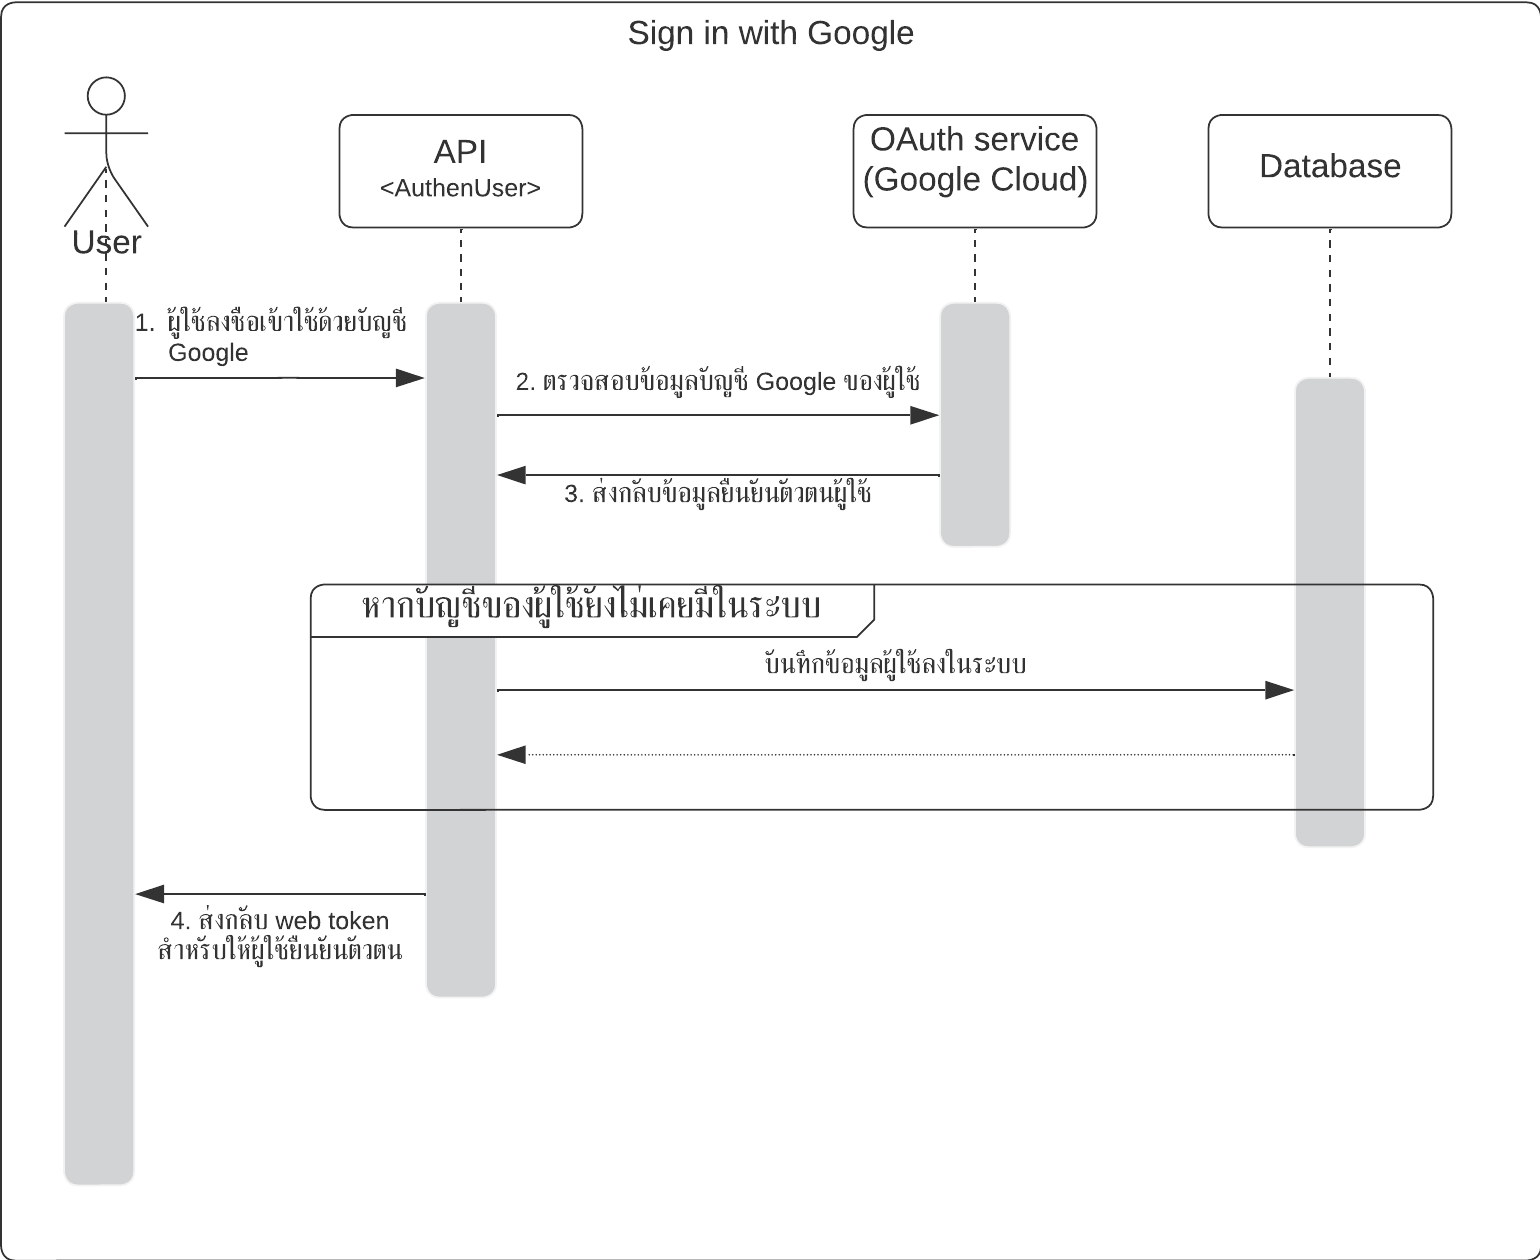
\includegraphics[width=8cm]{./figure/sequence-diagram/figure_sequence_sign_in.png}}
    \caption{Sign In with Google Sequence Diagram}\label{fig:signinSeqDiagram}
\end{figure}
\textbf{สถานการณ์: }ผู้ใช้ลงชื่อเข้าใช้ด้วยบัญชี Google
\begin{enumerate}
    \item ผู้ใช้ส่งคำขอลงชื่อเข้าใช้
    \item redirect ผู้ใช้ไปที่หน้าเลือกบัญชีของ Google
    \item ผู้ใช้เลือกบัญชี บริการ Google ส่งกลับข้อมูลบัญชีมานั้นที่ระบบหลังบ้าน
    \item หากบัญชีนี้ยังไม่เคยสมัครสมาชิกมาก่อน จะทำการบันทึกลงสู่ฐานข้อมูลด้วย
    \item ส่งกลับข้อมูลบัญชีและโทเคนกลับสู้ผู้ใช้งาน
\end{enumerate}

\subsection{Resume Prediction}
\begin{figure}[H]\centering
    \setlength{\fboxrule}{0.2mm} % can define this in the preamble
    \fbox{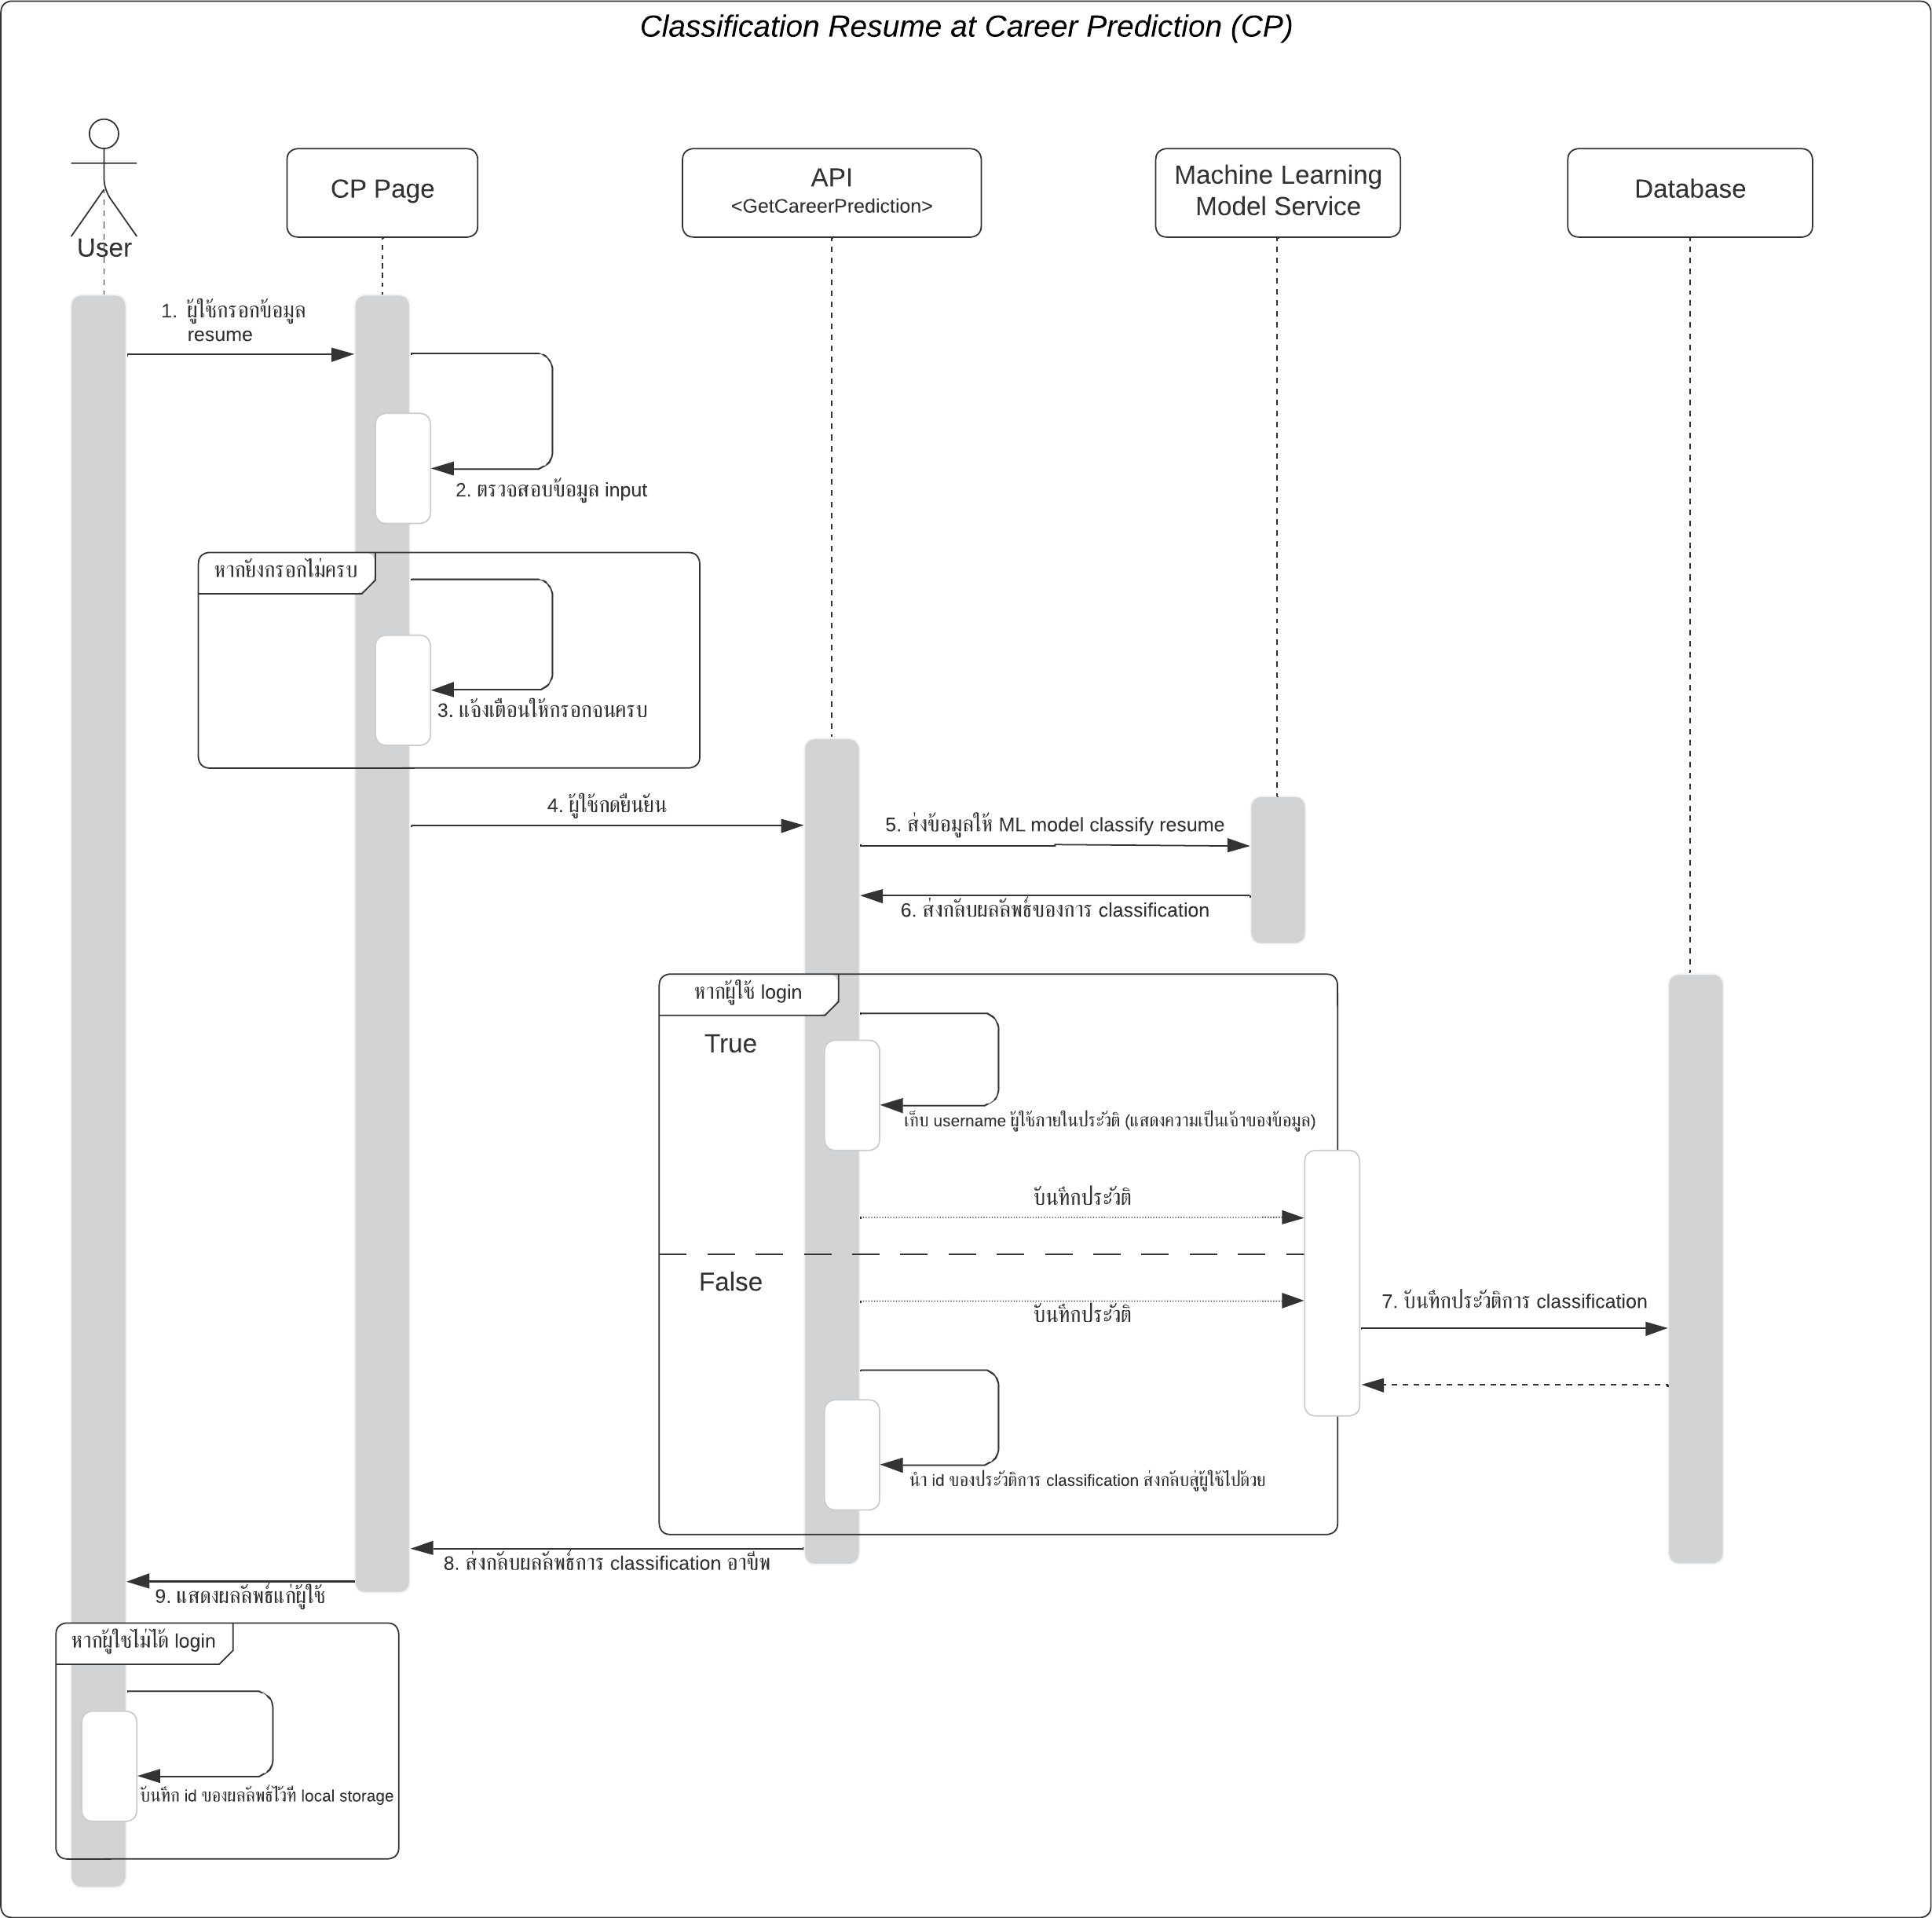
\includegraphics[width=8cm]{./figure/sequence-diagram/figure_sequence_prediction.png}}
    \caption{Resume Prediction Sequence Diagram}\label{fig:resumePredictSeqDiagram}
\end{figure}
\textbf{สถานการณ์: }ผู้ใช้ใช้งานระบบวิเคราะห์เรซูเม
\begin{enumerate}
    \item ผู้ใช้กรอกข้อมูลเรซูเมของตัวเอง
    \item user interface รับมือกรณีที่ผู้ใช้กรอกข้อมูลไม่ครบ และแจ้งเตือนแก่ผู้ใช้
    \item ผู้ใช้กรอกข้อมูลถูกต้องและส่งคำขอสู่บริการหลัก
    \item บริการหลักจัดการวิเคราะห์ข้อมูลเรซูเมของผู้ใช้ ผ่านการใช้บริการโมเดลปัญญาประดิษฐ์
    \item นำผลลัพธ์มาบันทึกลงสู่ฐานข้อมูล หากผู้ใช้งาน login อยู่ จะบันทึกชื่อของผู้ใช้ลงระบบไปด้วยเพื่อระบุตัวตน หากผู้ใช้ไม่ได้ login จะนำหมายเลขของประวัติส่งกลับผู้ใช้ไปด้วย
    \item ส่งข้อมูลกลับสู่ผู้ใช้งานและแสดงผล
\end{enumerate}

\subsection{Resume Insight}
\begin{figure}[H]\centering
    \setlength{\fboxrule}{0.2mm} % can define this in the preamble
    \fbox{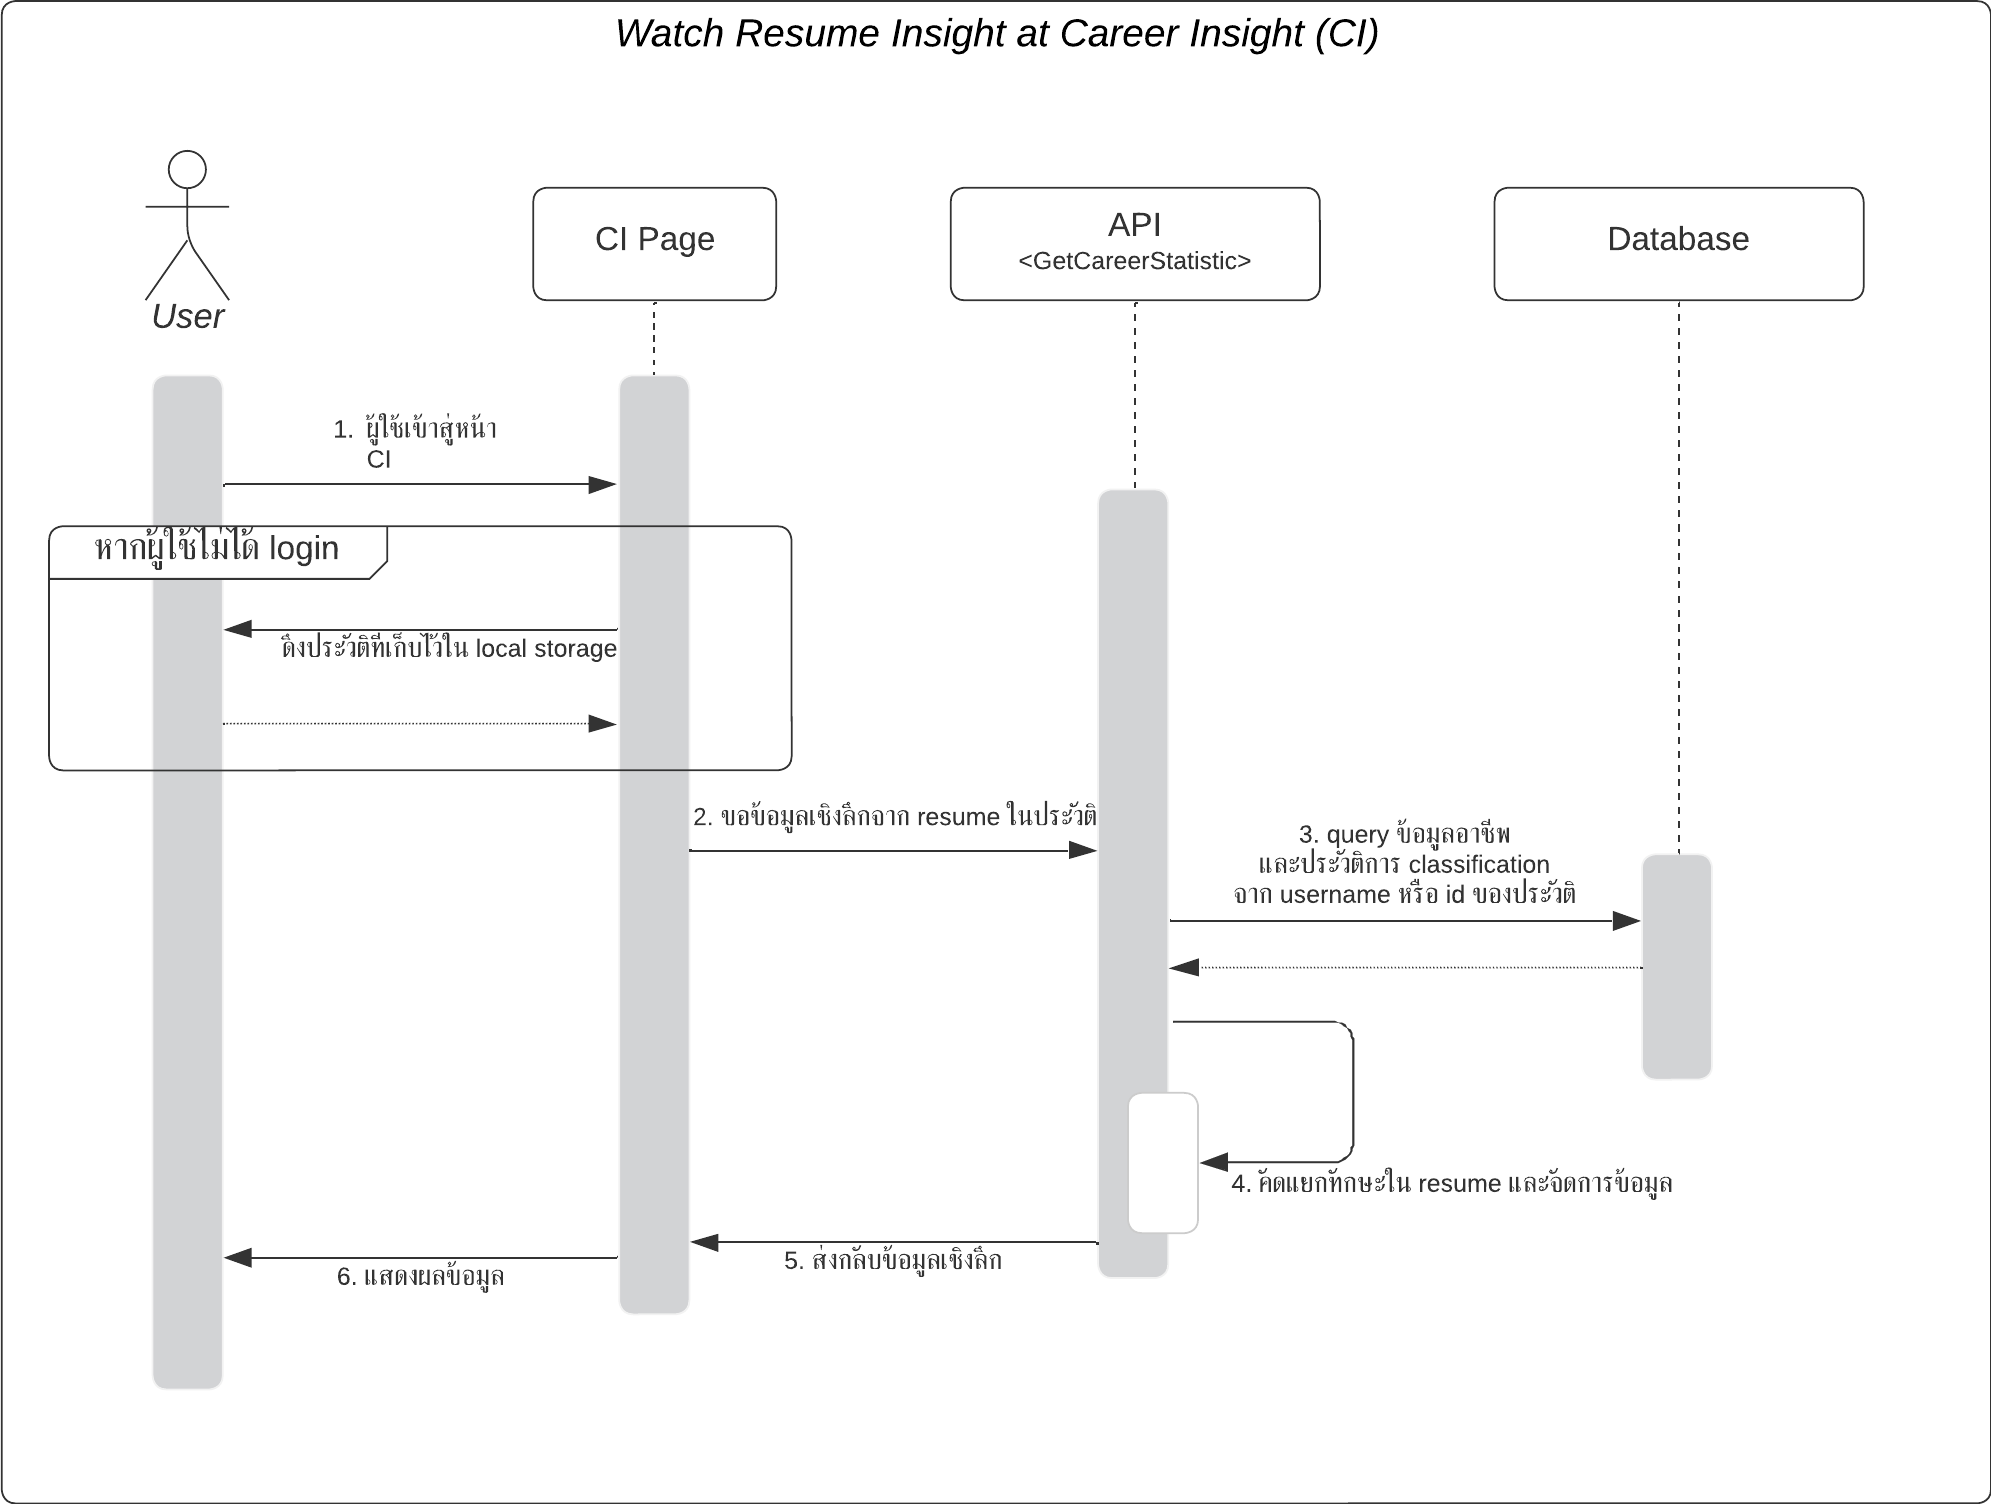
\includegraphics[width=8cm]{./figure/sequence-diagram/figure_sequence_insight.png}}
    \caption{Resume Insight Sequence Diagram}\label{fig:insightResumeSeqDiagram}
\end{figure}
\textbf{สถานการณ์: }ผู้ใช้เข้าดูข้อมูลเชิงลึกจากประวัติการวิเคราะห์เรซูเม
\begin{enumerate}
    \item หากผู้ใช้ login จะดึงประวัติการทำนายมาจากฐานข้อมูล หากไม่ใช่ จะนำมาจาก local storage ของผู้ใช้
    \item ผู้ใช้เข้าสู่หน้าวิเคราะห์ข้อมูลเชิงลึกจากช่องใดทางหนึ่ง เช่น ผ่านการ redirect จากหน้าวิเคราะห์เรซูเม หรือเข้าสู่หน้าข้อมูลเชิงลึกโดยตรง (ต้องมีข้อมูลมาก่อน)
    \item ระบบหน้าบ้าน ส่งคำขอสู่ระบบบริการหลัก เพื่อวิเคราะห์ข้อมูลจากเรซูเมนั้น ๆ
    \item บริการหลักคำนวณข้อมูลและส่งกลับสู่ผู้ใช้
    \item แสดงผลแก่ผู้ใช้
\end{enumerate}

\subsection{Watch Career Exploration}
\begin{figure}[H]\centering
    \setlength{\fboxrule}{0.2mm} % can define this in the preamble
    \fbox{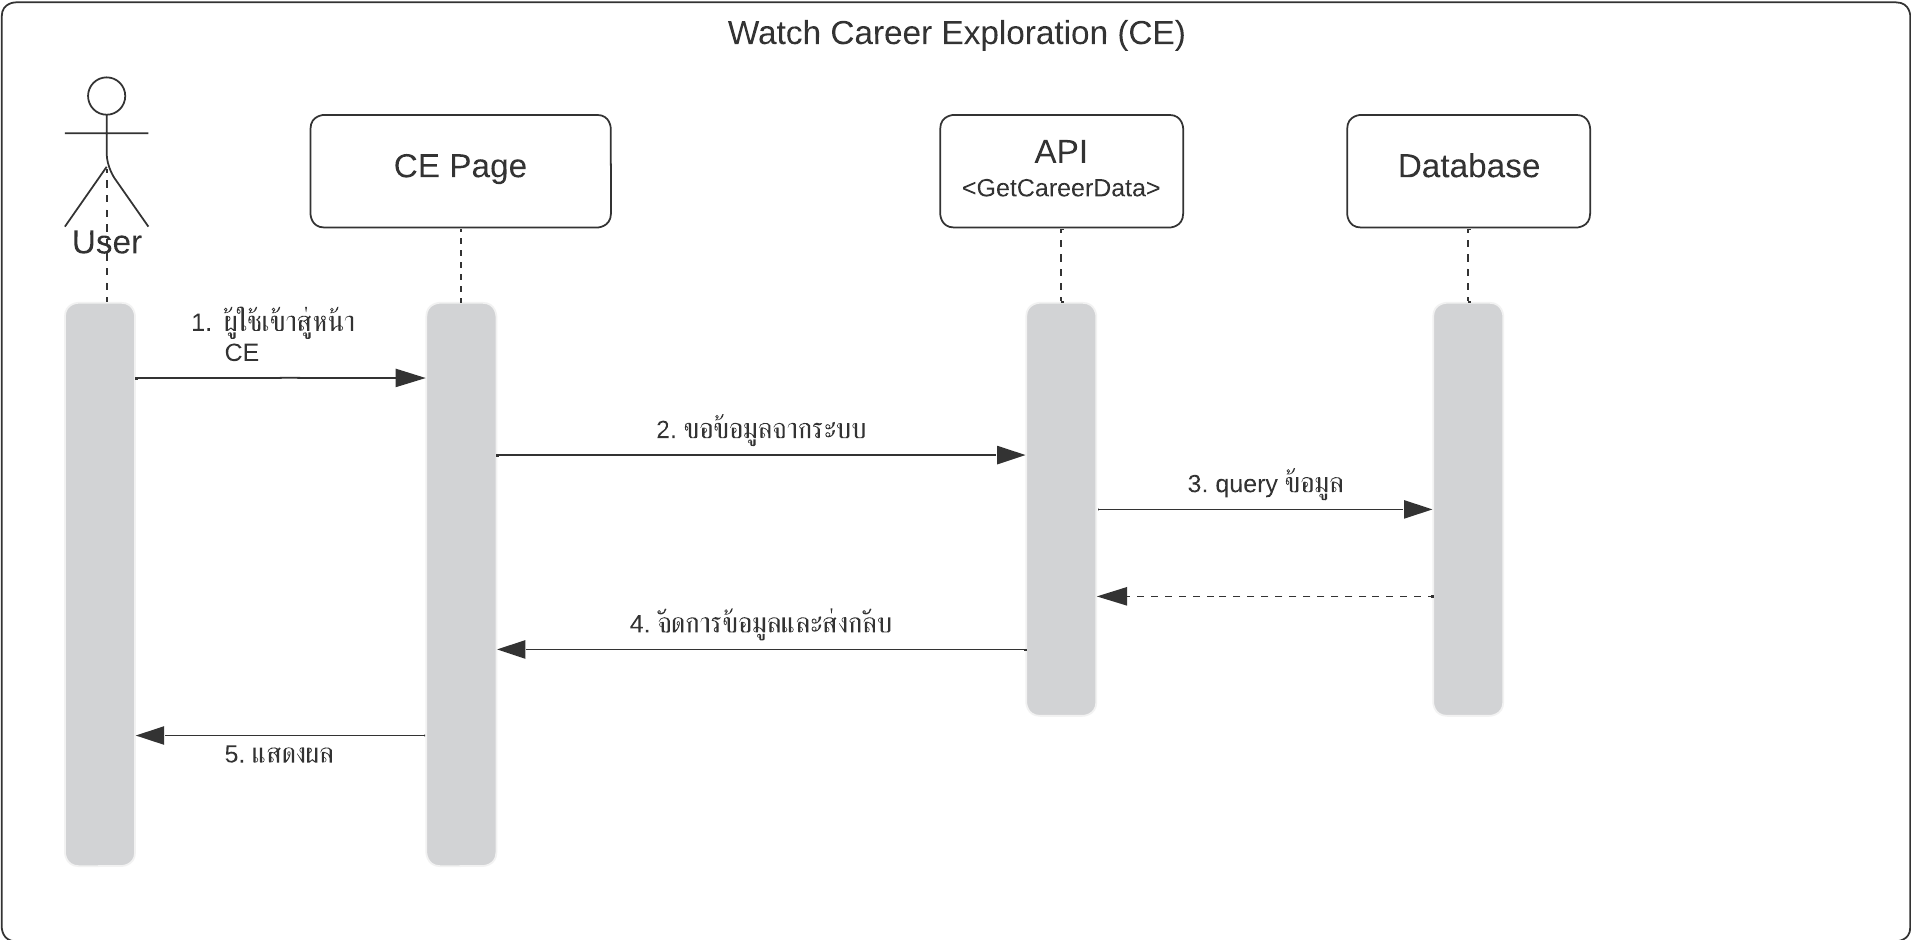
\includegraphics[width=8cm]{./figure/sequence-diagram/figure_sequence_exploration.png}}
    \caption{Watch Career Exploration Sequence Diagram}\label{fig:exploreSeqDiagram}
\end{figure}
\textbf{สถานการณ์: }ผู้ใช้เข้าดูหน้าสายใยอาชีพ
\begin{enumerate}
    \item ผู้ใช้เข้าสู่หน้าสายใยอาชีพ
    \item ระบบหน้าบ้านขอข้อมูลจากบริการหลักและดึงข้อมูลจากฐานข้อมูล
    \item บริการหลักส่งข้อมูลกลับสู่ผู้ใช้และแสดงผล
\end{enumerate}

%%%%%%%%%%%%%%%%%%%%%%%%%%%%%%%%%%%%%%%%%%%%%%%%%%%%%%%%%%%%%
% Database structure Section
%%%%%%%%%%%%%%%%%%%%%%%%%%%%%%%%%%%%%%%%%%%%%%%%%%%%%%%%%%%%%


\section{Database}
ระบบฐานข้อมูลของเราจะใช้เป็นรูปแบบ NoSQL ประเภท document ผ่านบริการของ MongoDB โดยมีรายละเอียดในแต่ละตาราง ดังนี้
\begin{figure}[H]\centering
    \setlength{\fboxrule}{0.2mm} % can define this in the preamble
    \setlength{\fboxsep}{0.5cm}
    \fbox{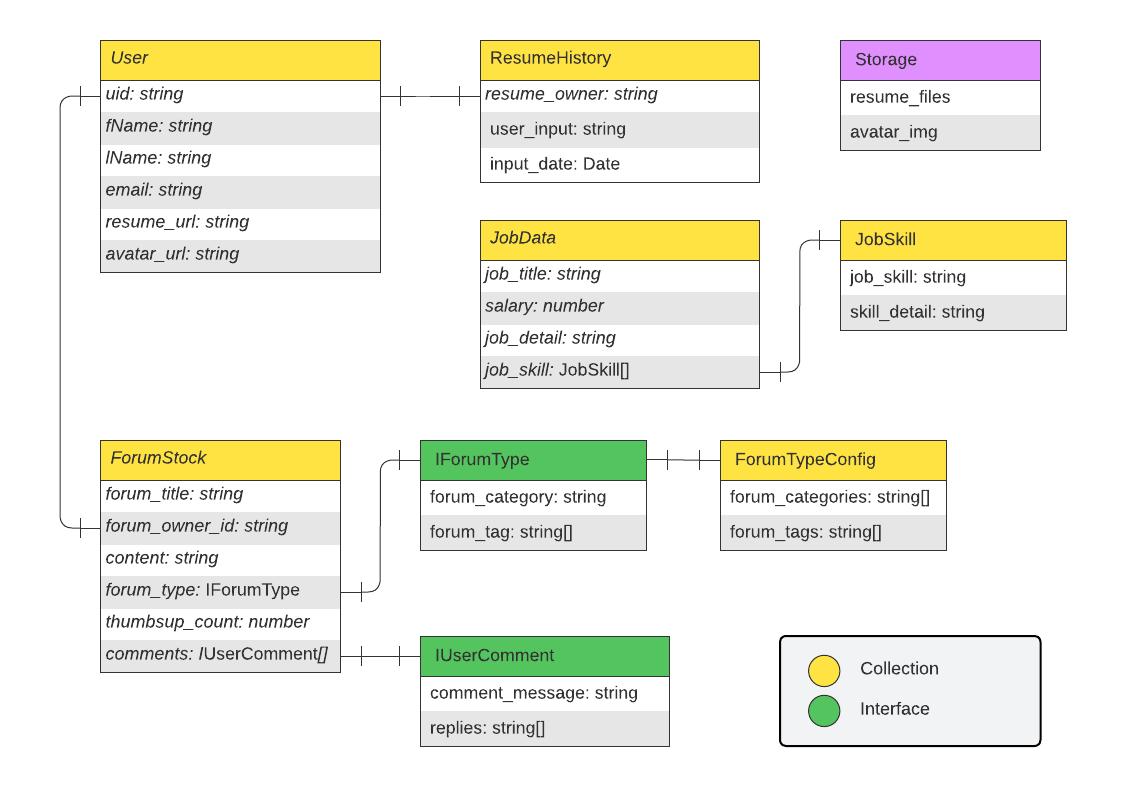
\includegraphics[width=8cm]{./figure/figure_database.png}}
    \caption{Database Structure}\label{fig:database}
\end{figure}

\subsection{ตารางฐานข้อมูล User}
\begin{table}[H]
    \begin{tabularx}{\textwidth}{|l|l|X|}
        \hline
        \multicolumn{3}{|c|}{User}                                                                                                      \\ \hline
        Field Name  & Field Type & Description                                                                                        \\ \hline
        uid         & string     & รหัสประจำตัวของผู้ใช้ ที่ทางระบบจะเป็นผู้กำหนดให้ เพื่อใช้แยกผู้ใช้แต่ละท่านอย่างชัดเจน            \\
        firstname   & string     & ชื่อต้นของผู้ใช้                                                                                   \\
        lastname    & string     & นามสกุลของผู้ใช้                                                                                   \\
        email       & string     & อีเมลของผู้ใช้                                                                                     \\
        image\_url  & string     & url สำหรับเข้าถึงรูปโปรไฟล์ของผู้ใช้ \\ \hline
    \end{tabularx}
\end{table}

\subsection{ตารางฐานข้อมูล ResumeHistory}
\begin{table}[H]
    \begin{tabularx}{\textwidth}{|l|l|X|}
        \hline
        \multicolumn{3}{|c|}{ResumeHistory}                                                                   \\\hline
        Field Name    & Field Type & Description                                                            \\\hline
        resume\_owner & string     & รหัสประจำตัวของผู้ใช้ รูปแบบเดียวกับ uid ใช้สำหรับการระบุเจ้าของข้อมูล \\
        resume\_input   & IResumeInput     & ค่าเรซูเมรับเข้าจากผู้ใช้ โดยมีลักษณะข้อมูลดังภาพ ประกอบด้วย การศึกษา ความสามารถ ประสบการณ์ \\
        input\_date   & Date       & วันที่ผู้ใช้กรอกข้อมูล \\ \hline
    \end{tabularx}
\end{table}

\subsection{ตารางฐานข้อมูล Career Path Data}
\begin{table}[H]
    \begin{tabularx}{\textwidth}{|l|l|X|}
        \hline
        \multicolumn{3}{|c|}{Career Path Data}                                                                      \\\hline
        Field Name  & Field Type     & Description                                                       \\\hline
        career\_path\_name             & string         & ชื่อของอาชีพ                                                      \\
        career\_path\_description      & string         & ข้อมูลเบื้องต้นของอาชีพนั้น เพื่ออธิบายลักษณะของสายอาชีพให้เห็นภาพโดยง่าย \\
        related\_careers              & IRelatedCareer{[}{]} &   อาชีพที่อยู่ในสายอาชีพนั้น ๆ และข้อมูลเบื้องต้น เช่น ชื่ออาชีพ ความสามารถ ทักษะที่ควรมี \\
        base\_salary                   & IBaseSalary & ฐานเงินเดือนของอาชีพนั้นโดยเป็น object ที่จะเก็บขอบเขตเงินเดือนเอาไว้ \\ \hline
    \end{tabularx}
\end{table}

\subsection{ตารางฐานข้อมูล Skill Domain}
\begin{table}[H]
    \begin{tabularx}{\textwidth}{|l|l|X|}
        \hline
        \multicolumn{3}{|c|}{Skill Domain}                              \\\hline
        Field Name    & Field Type & Description                  \\\hline
        id    & string     & หมายเลขจำเพาะของกลุ่มความสามารถที่ควรในประเภทเดียวกัน       \\
        name & string     & ชื่อของกลุ่มความสามารถในประเภทเดียวกัน เช่น basic web development \\
        skill\_list    & string[]     & ชุดของความสามารถที่อยู่ในกลุ่มนี้ ภายในจะเก็บ id ของความสามารถเอาไว้       \\
        is\_in\_resume & boolean     & ตัวแปรสำหรับกำหนดว่า ความสามารถนี้เป็นสิ่งจำเป็น แต่อาจไม่จำเป็นต้องเขียนในเรซูเมใช่หรือไม่ เพื่อนำไปทำเป็นเงื่อนไขการแสดงผล \\\hline
    \end{tabularx}
\end{table}

\subsection{ตารางฐานข้อมูล Skill Data}
\begin{table}[H]
    \begin{tabularx}{\textwidth}{|l|l|X|}
        \hline
        \multicolumn{3}{|c|}{Skill Data}                              \\\hline
        Field Name    & Field Type & Description                  \\\hline
        id    & string     & หมายเลขจำเพาะของความามารถนี้       \\
        name  & string[]   & ชื่อของความสามารถ \\ \hline
    \end{tabularx}
\end{table}

%%%%%%%%%%%%%%%%%%%%%%%%%%%%%%%%%%%%%%%%%%%%%%%%%%%%%%%%%%%%%
% Site Map Section
%%%%%%%%%%%%%%%%%%%%%%%%%%%%%%%%%%%%%%%%%%%%%%%%%%%%%%%%%%%%%

\section{แผนผังเว็บไซต์ (Site Map)}
แผนผังเว็บไซต์ (Site Map) เป็นโครงสร้างแบบภาพรวมที่แสดงถึงโครงสร้างของเว็บไซต์ทั้งหมด ซึ่งมีวัตถุประสงค์หลักคือการให้ผู้ใช้และเครื่องมือการค้นหาเข้าใจโครงสร้างและลำดับของเนื้อหาบนเว็บไซต์ได้ง่ายขึ้น แผนผังเว็บไซต์ช่วยในการนำทางผู้ใช้ไปสู่ส่วนต่าง ๆ ของเว็บไซต์, ลดความสับสนและเพิ่มประสิทธิภาพในการค้นหาข้อมูล

\begin{figure}[H]\centering
    \setlength{\fboxrule}{0.2mm} % can define this in the preamble
    \setlength{\fboxsep}{0.5cm}
    \fbox{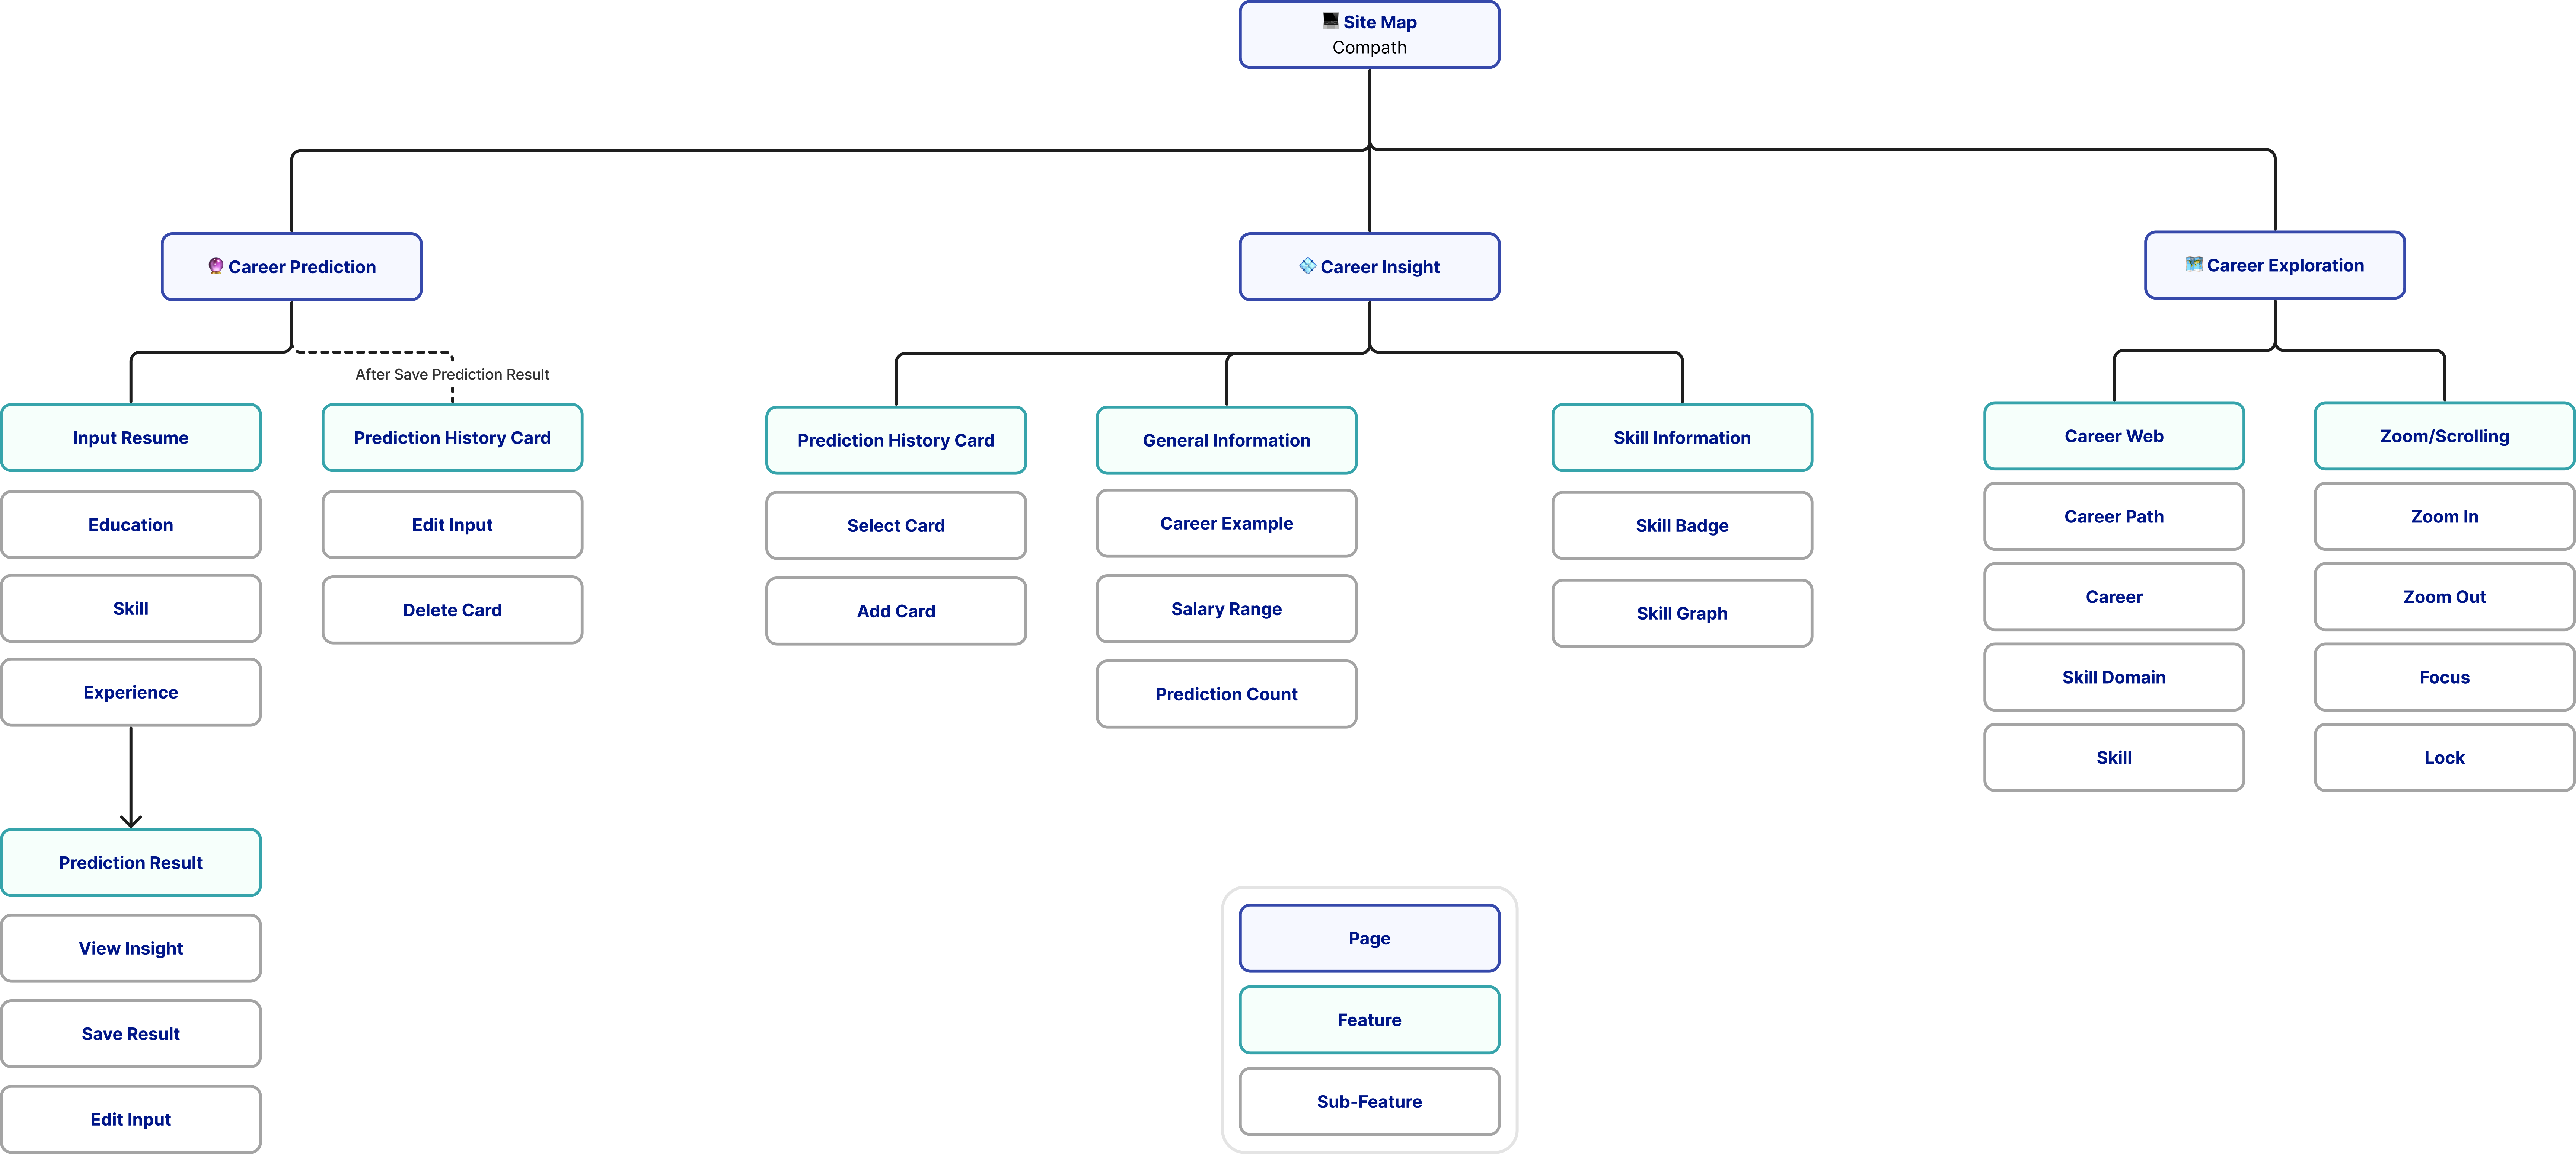
\includegraphics[width=14cm]{./figure/figure_siteMap.png}}
    \caption{Site Map}\label{fig:siteMap}
\end{figure}

%%%%%%%%%%%%%%%%%%%%%%%%%%%%%%%%%%%%%%%%%%%%%%%%%%%%%%%%%%%%%
% Navigation Map Section
%%%%%%%%%%%%%%%%%%%%%%%%%%%%%%%%%%%%%%%%%%%%%%%%%%%%%%%%%%%%%

\section{แผนที่การนำทางเว็บไซต์ (Navigation Map)}
แผนที่การนำทางเว็บไซต์ (Navigation Map) เป็นเครื่องมือที่ใช้ในการอธิบายหรือแสดงภาพรวมของโครงสร้างของเว็บไซต์ที่มีหลายหน้า โดยจุดประสงค์หลักของ Navigation Map คือการช่วยผู้ใช้ในการเข้าใจโครงสร้างและลำดับขั้นตอนในการนำทางภายในระบบ
\begin{figure}[H]\centering
    \fbox{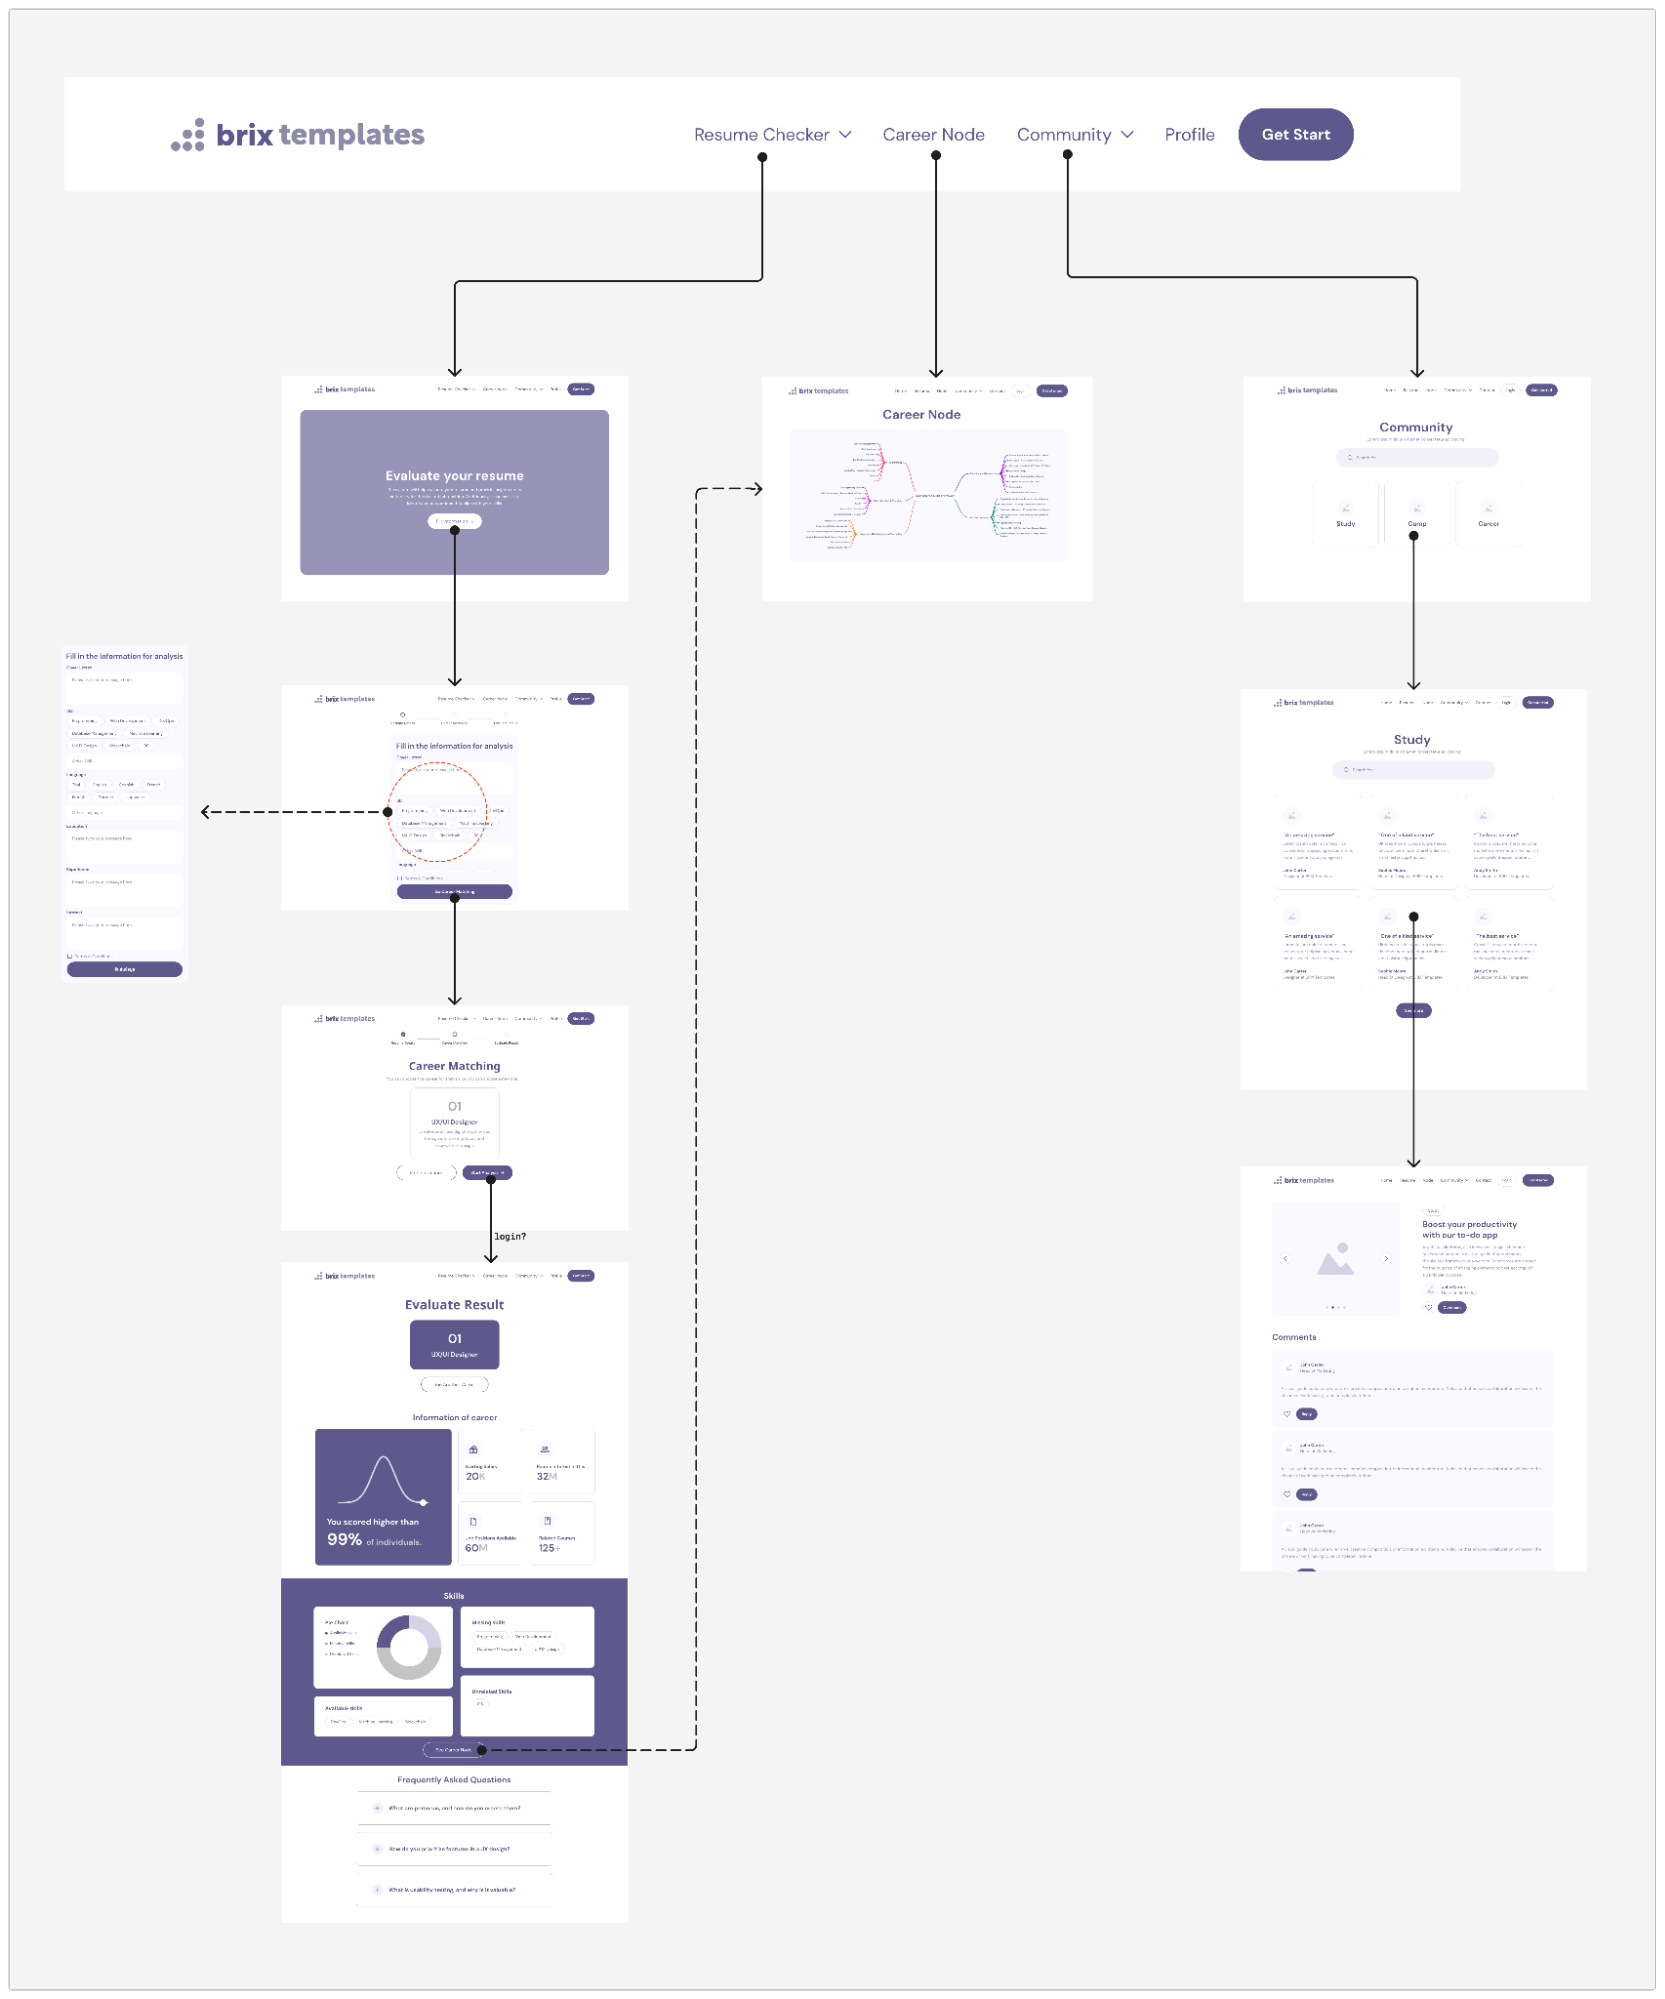
\includegraphics[width=14cm]{./figure/figure_navMap.png}}
    \caption{Navigation Map}\label{fig:navMap}
\end{figure}
\newpage

\section{การออกแบบส่วนต่อประสานกับผู้ใช้ (User Interface Design)}

\subsection{Career Prediction (ทํานายสายอาชีพ)}
คือหน้าสำหรับการทำนายสายอาชีพ ผู้ใช้จะต้องกรอกข้อมูลเพื่อให้ระบบนำข้อมูลไปทํานายสายอาชีพโดยผู้ใช้สามารถดูข้อมูลเบื่องต้นของอาชีพที่ทำนายได้ รวมถึงผู้ใช้สามารถดูประวัติการทำนายได้จากหน้านี้ ดังรูป \ref{fig:CP.png} - \ref{fig:CP-result.png} ดังนี้
\begin{figure}[H]\centering
    \fbox{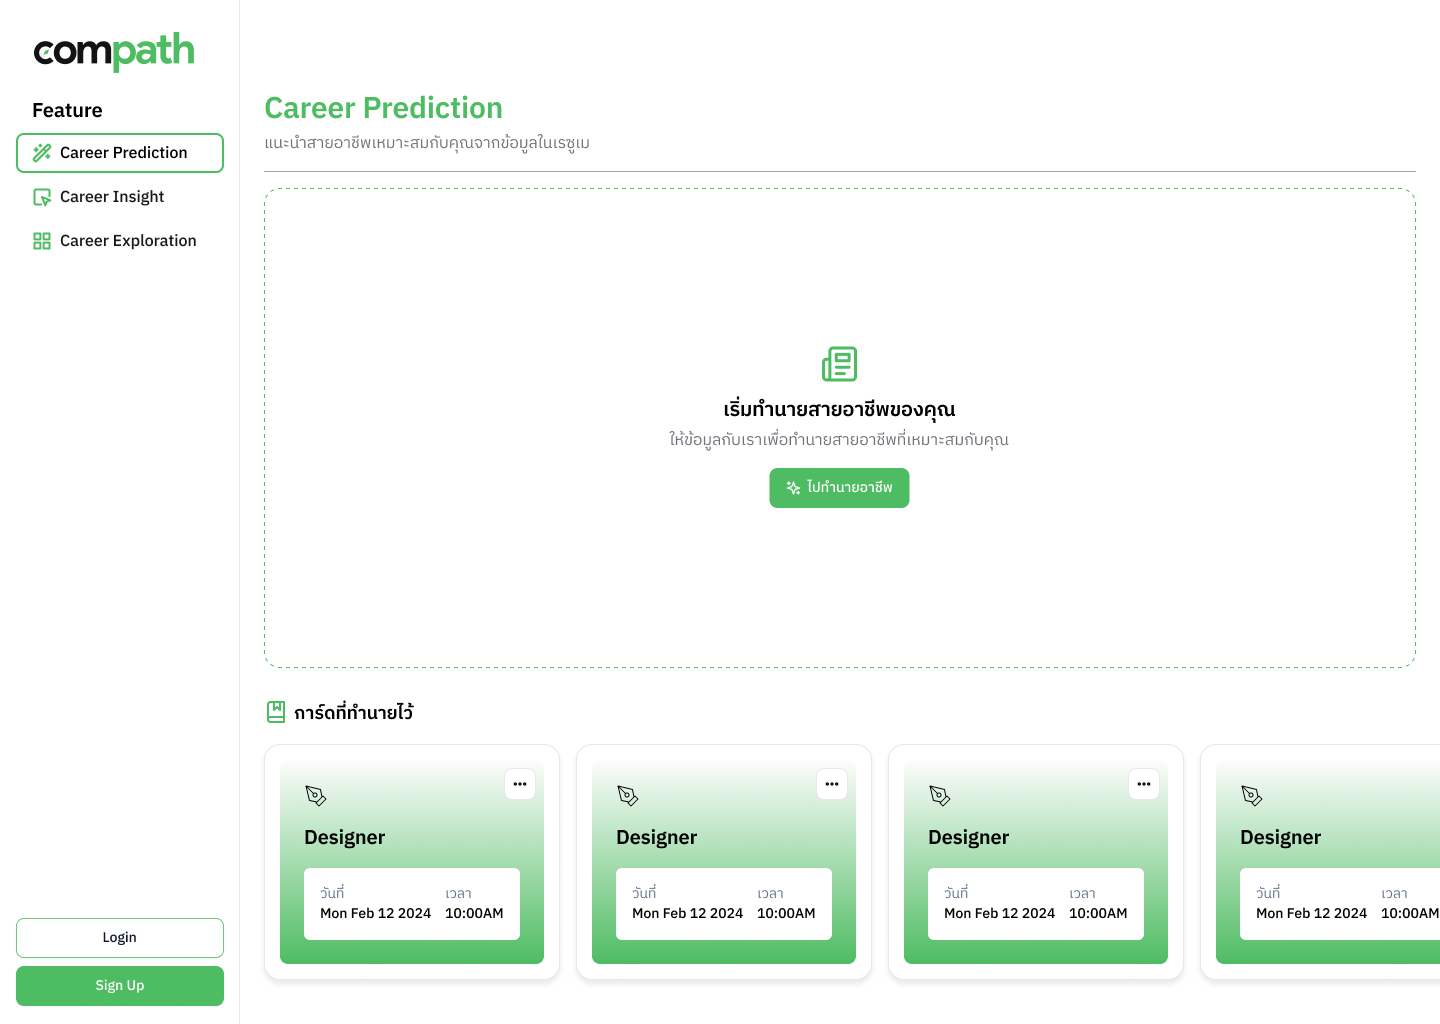
\includegraphics[width=12cm]{./figure/UI-picture/CP.png}}
    \caption{รูปแสดงการออกแบบหน้าทำนายสายอาชีพ}\label{fig:CP.png}
\end{figure}
\begin{figure}[H]\centering
    \fbox{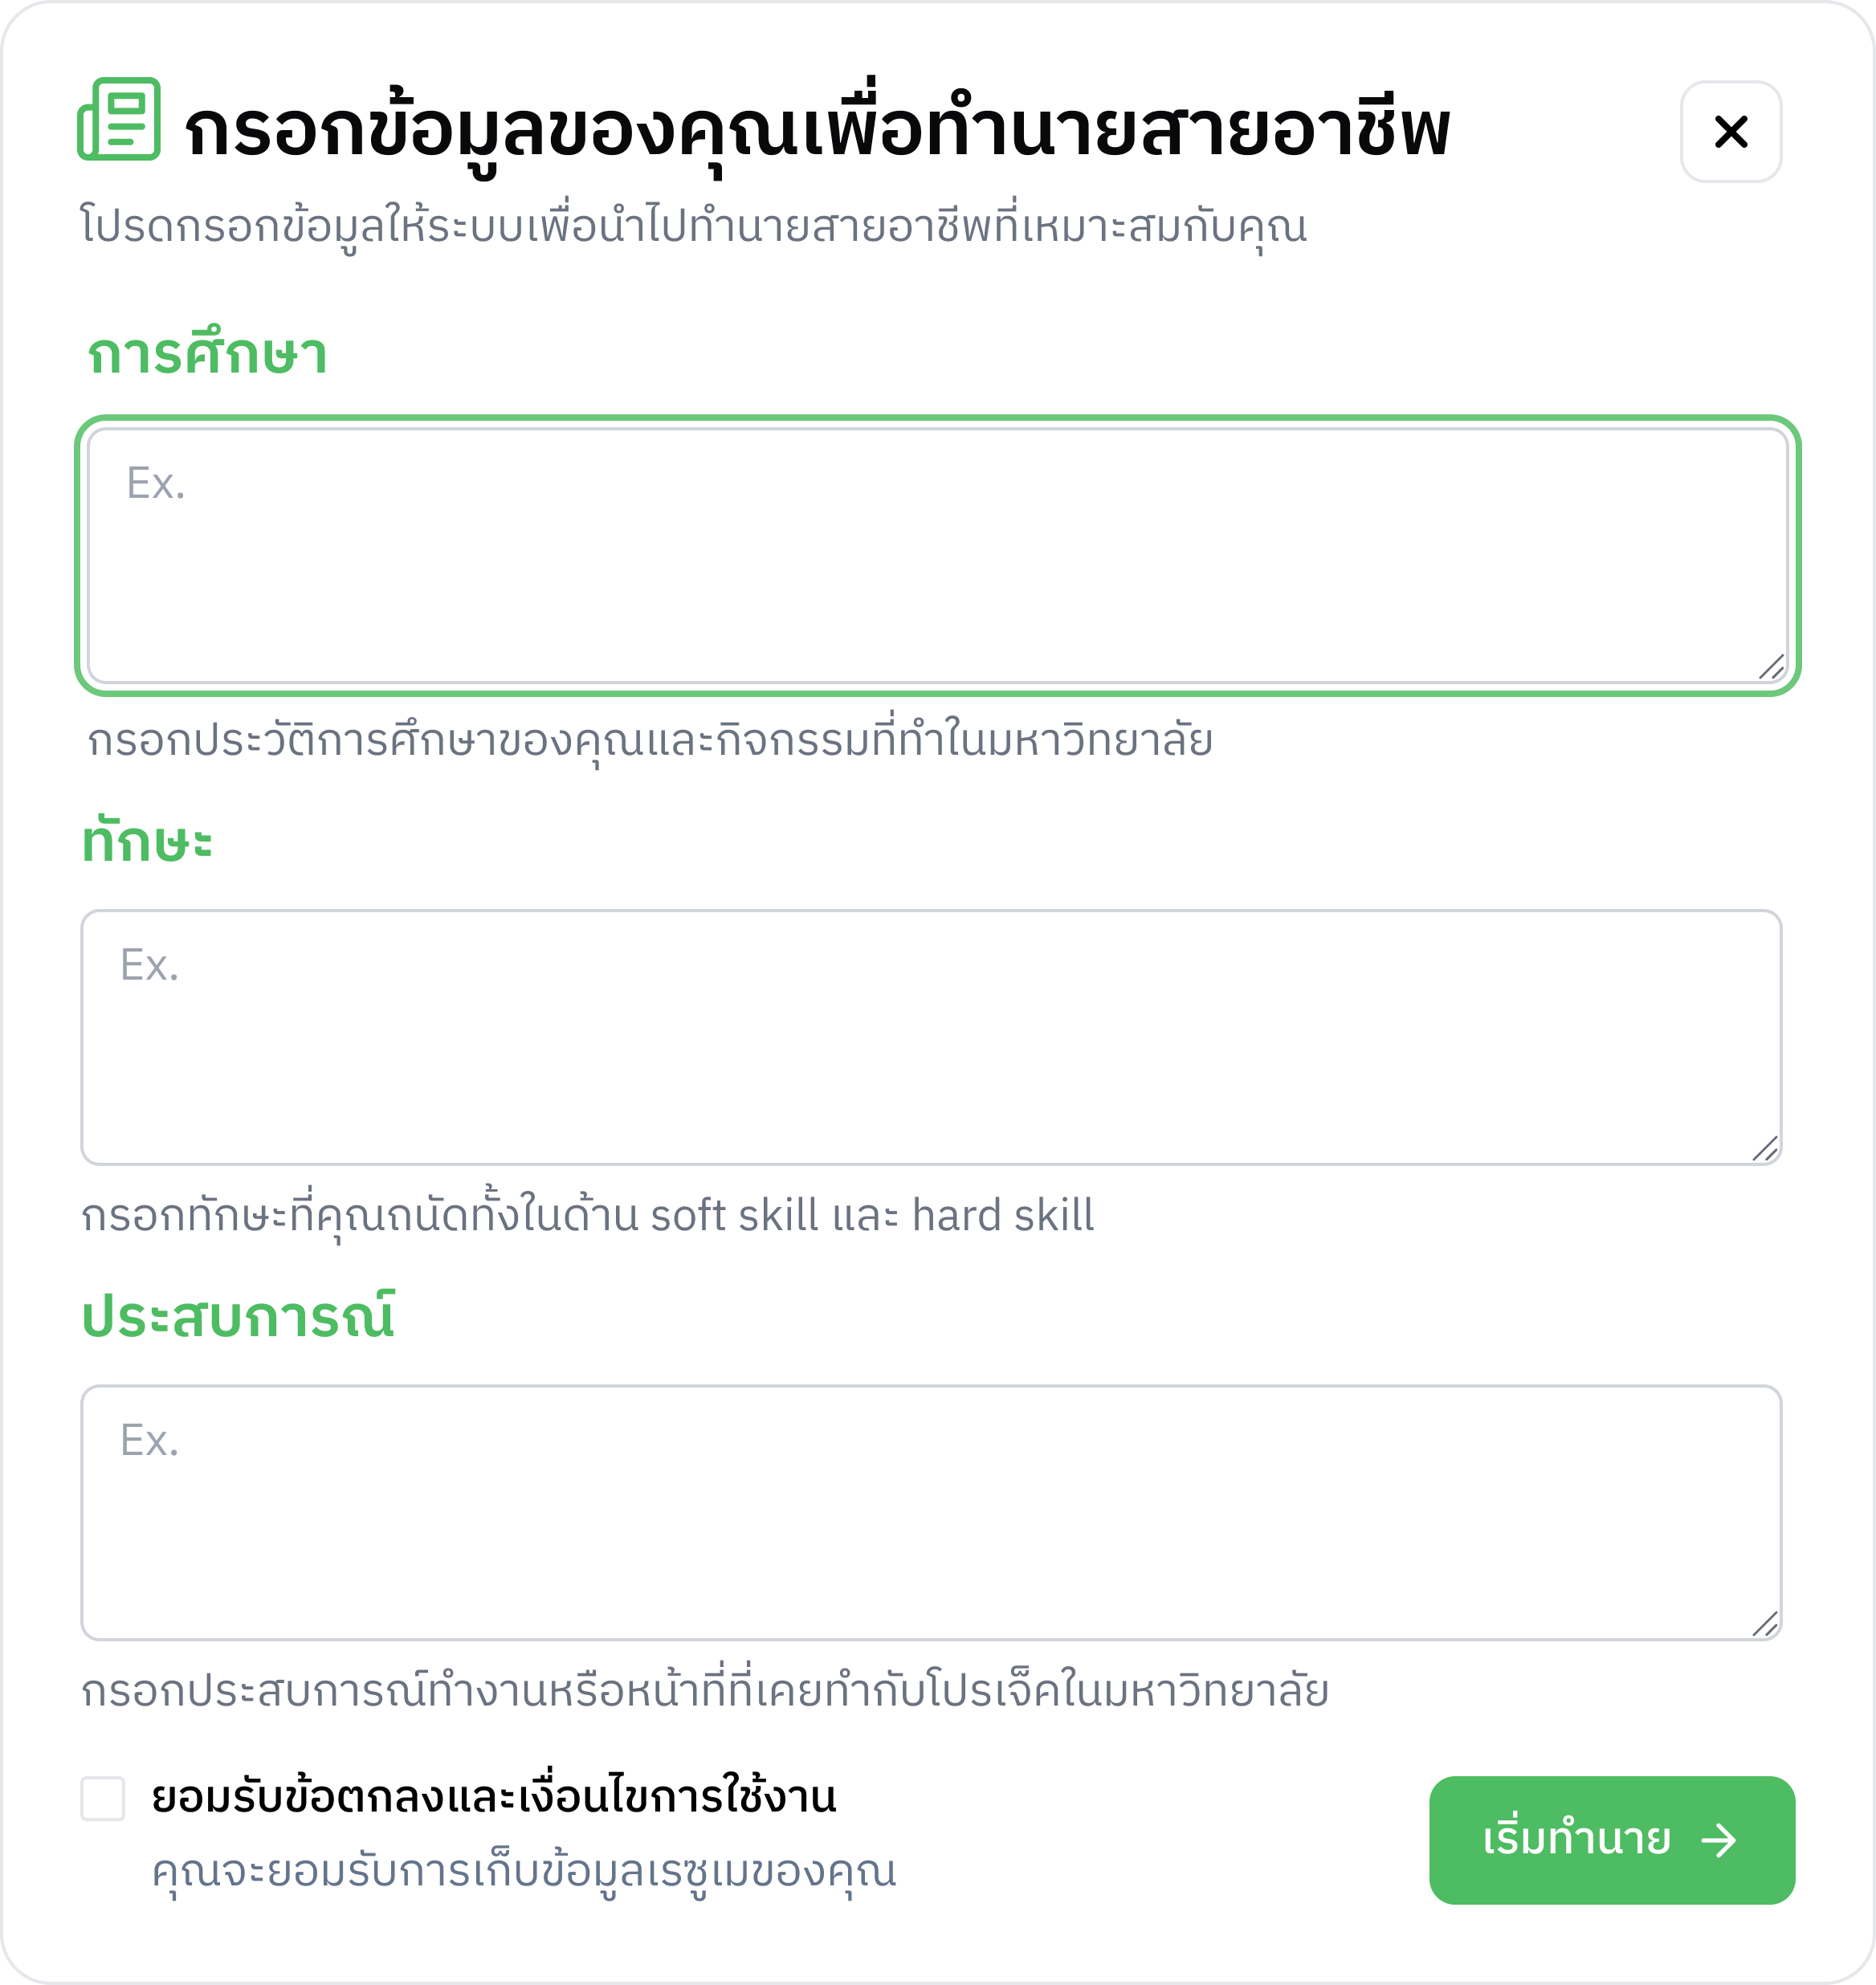
\includegraphics[width=8cm]{./figure/UI-picture/CP-input.png}}
    \caption{รูปแสดงการออกแบบหน้ากรอกข้อมูลเพื่อทำนายสายอาชีพ}\label{fig:CP-input.png}
\end{figure}
\begin{figure}[H]\centering
    \fbox{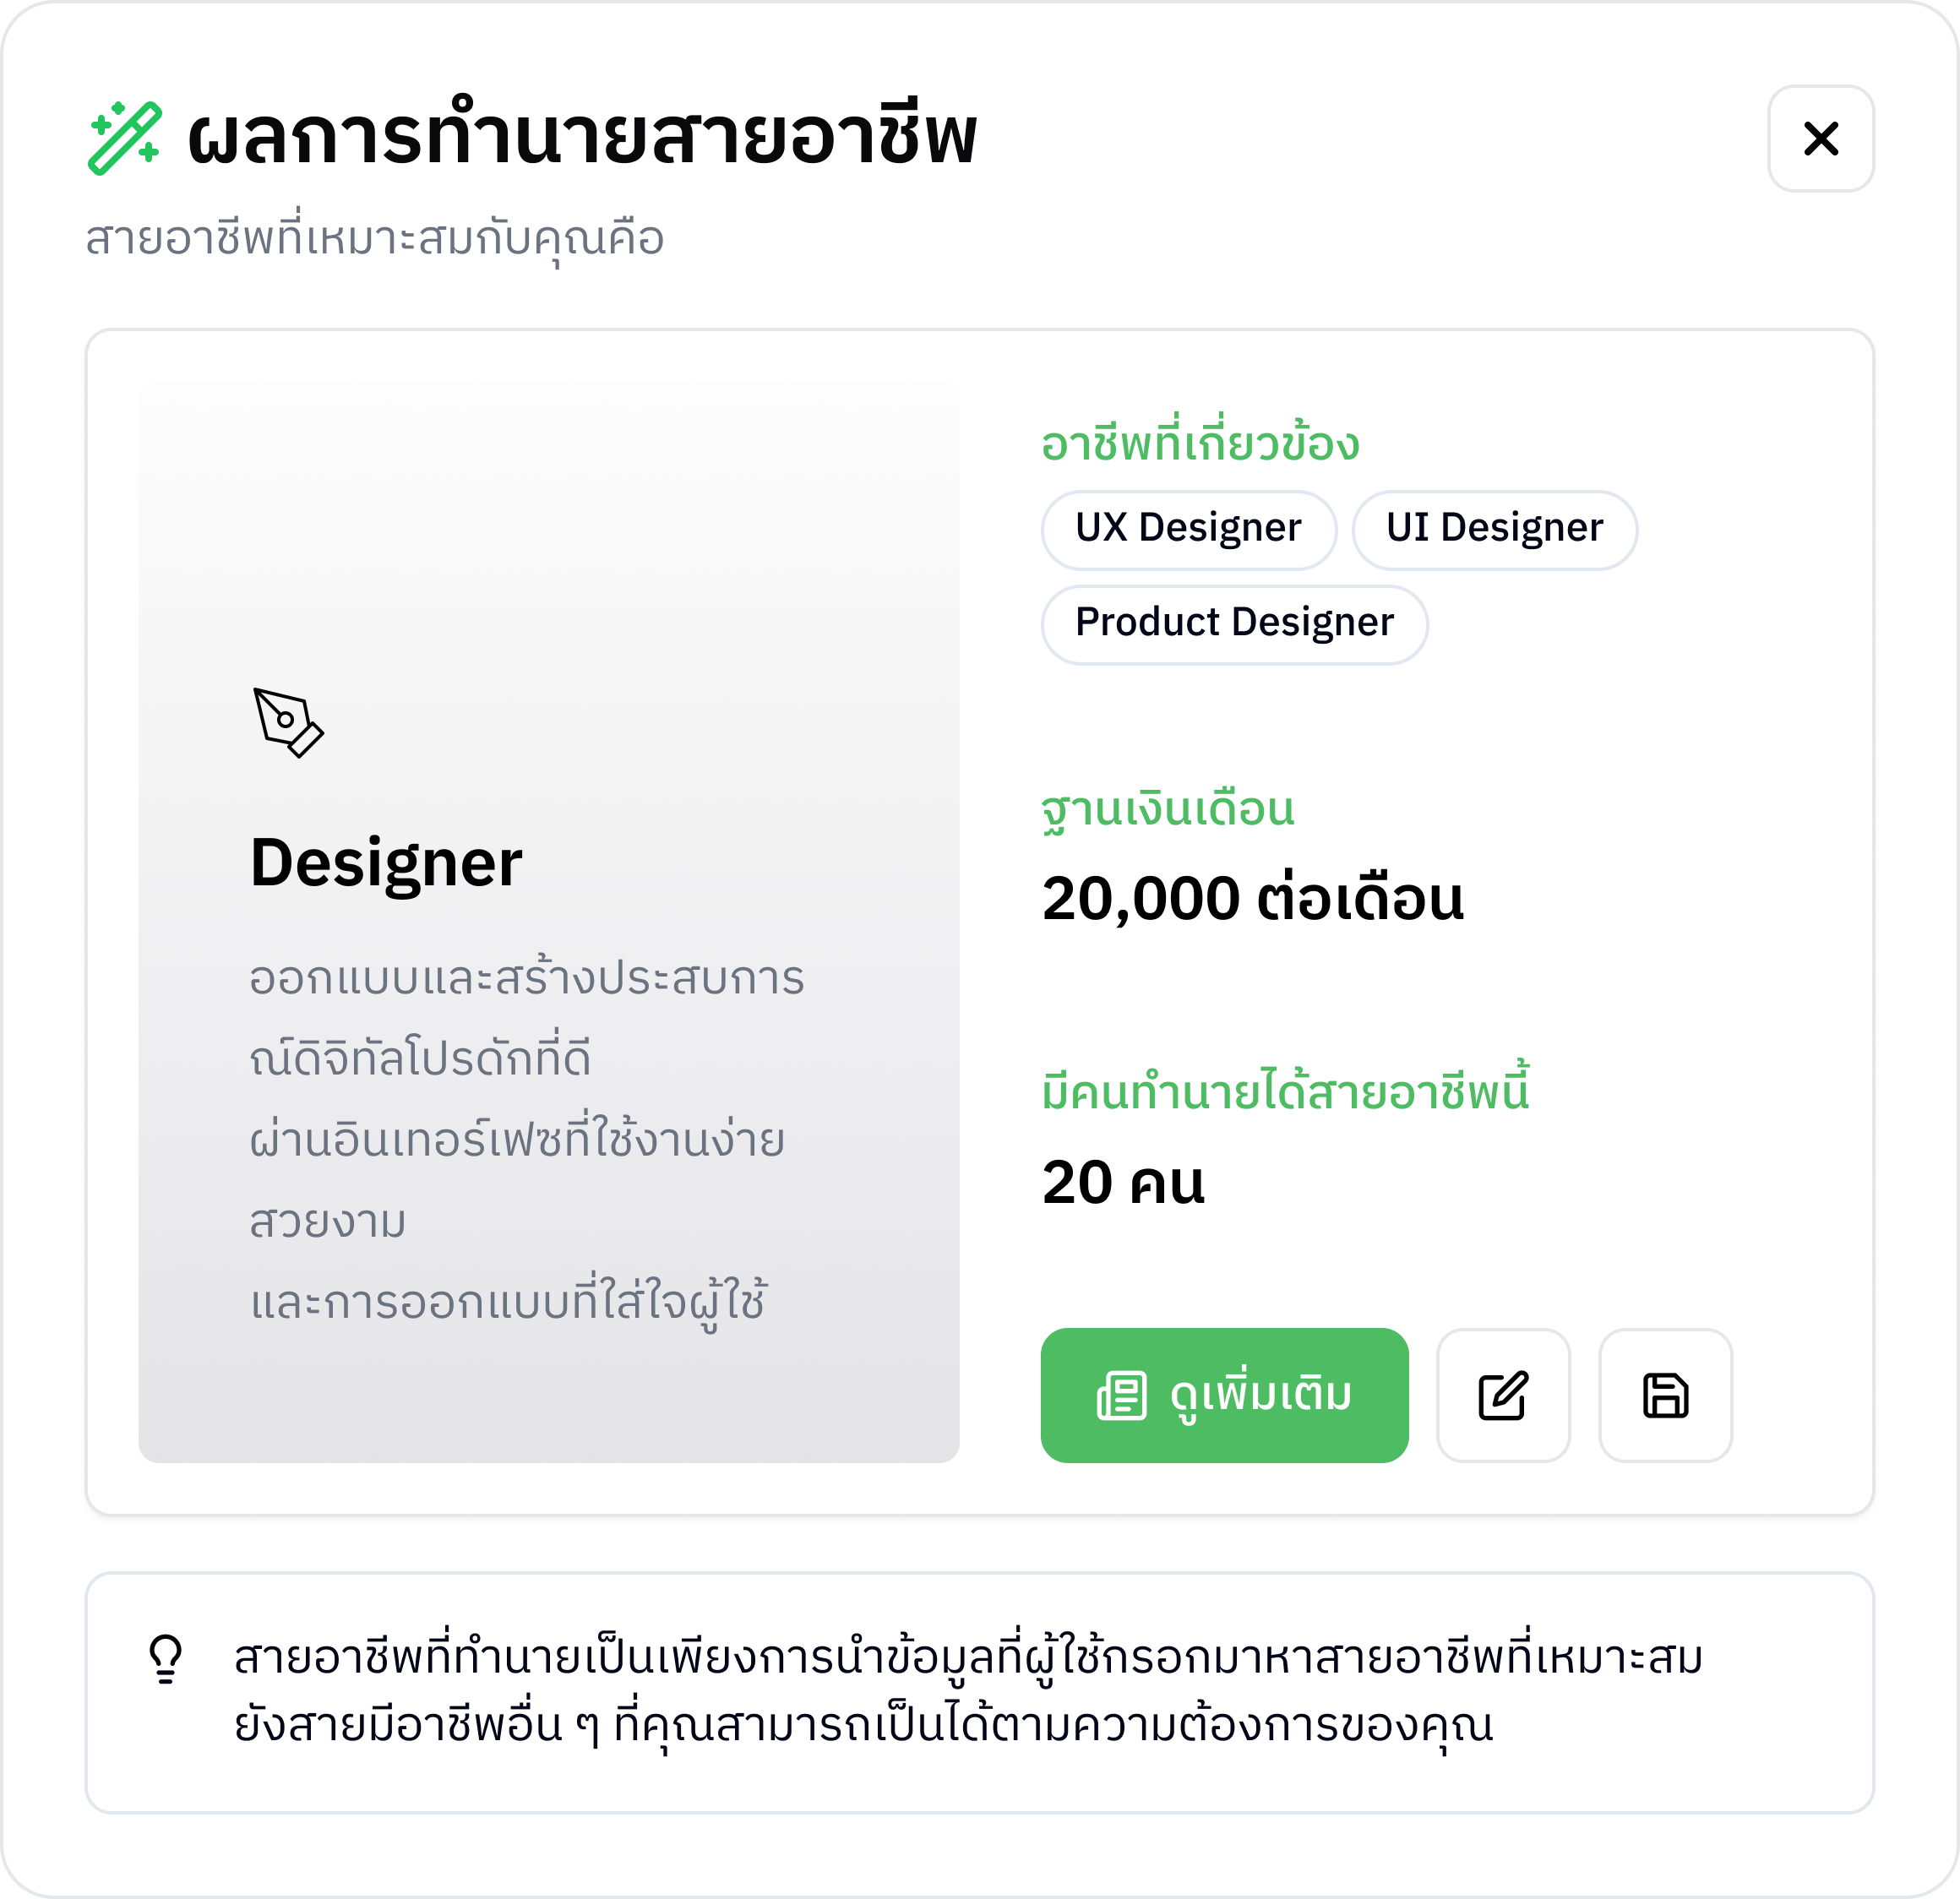
\includegraphics[width=8cm]{./figure/UI-picture/CP-result.png}}
    \caption{รูปแสดงการออกแบบหน้าผลลัพธ์การทำนายสายอาชีพ}\label{fig:CP-result.png}
\end{figure}

\subsection{Career Insight (ข้อมูลเชิงลึกของสายอาชีพ)}
คือหน้าสำหรับดูข้อมูลเชิงลึกของสายอาชีพที่ผู้ใช้เคยทำนายได้ โดยจะบอกทั้งในส่วนของข้อมูลเบื่องต้น เช่น ตัวอย่างของอาชีพที่เกี่ยวข้อง เงินเดือน จำนวนคนที่ทำนายได้สายอาชีพนี้เหมือนกัน เป็นต้น รวมถึงแสดงข้อมูลทักษะที่มักจะมีอยู่ในเรซูเมของสายอาชีพ ดังรูป \ref{fig:CI.png} - \ref{fig:CI-dropdown.png} ดังนี้
\begin{figure}[H]\centering
    \fbox{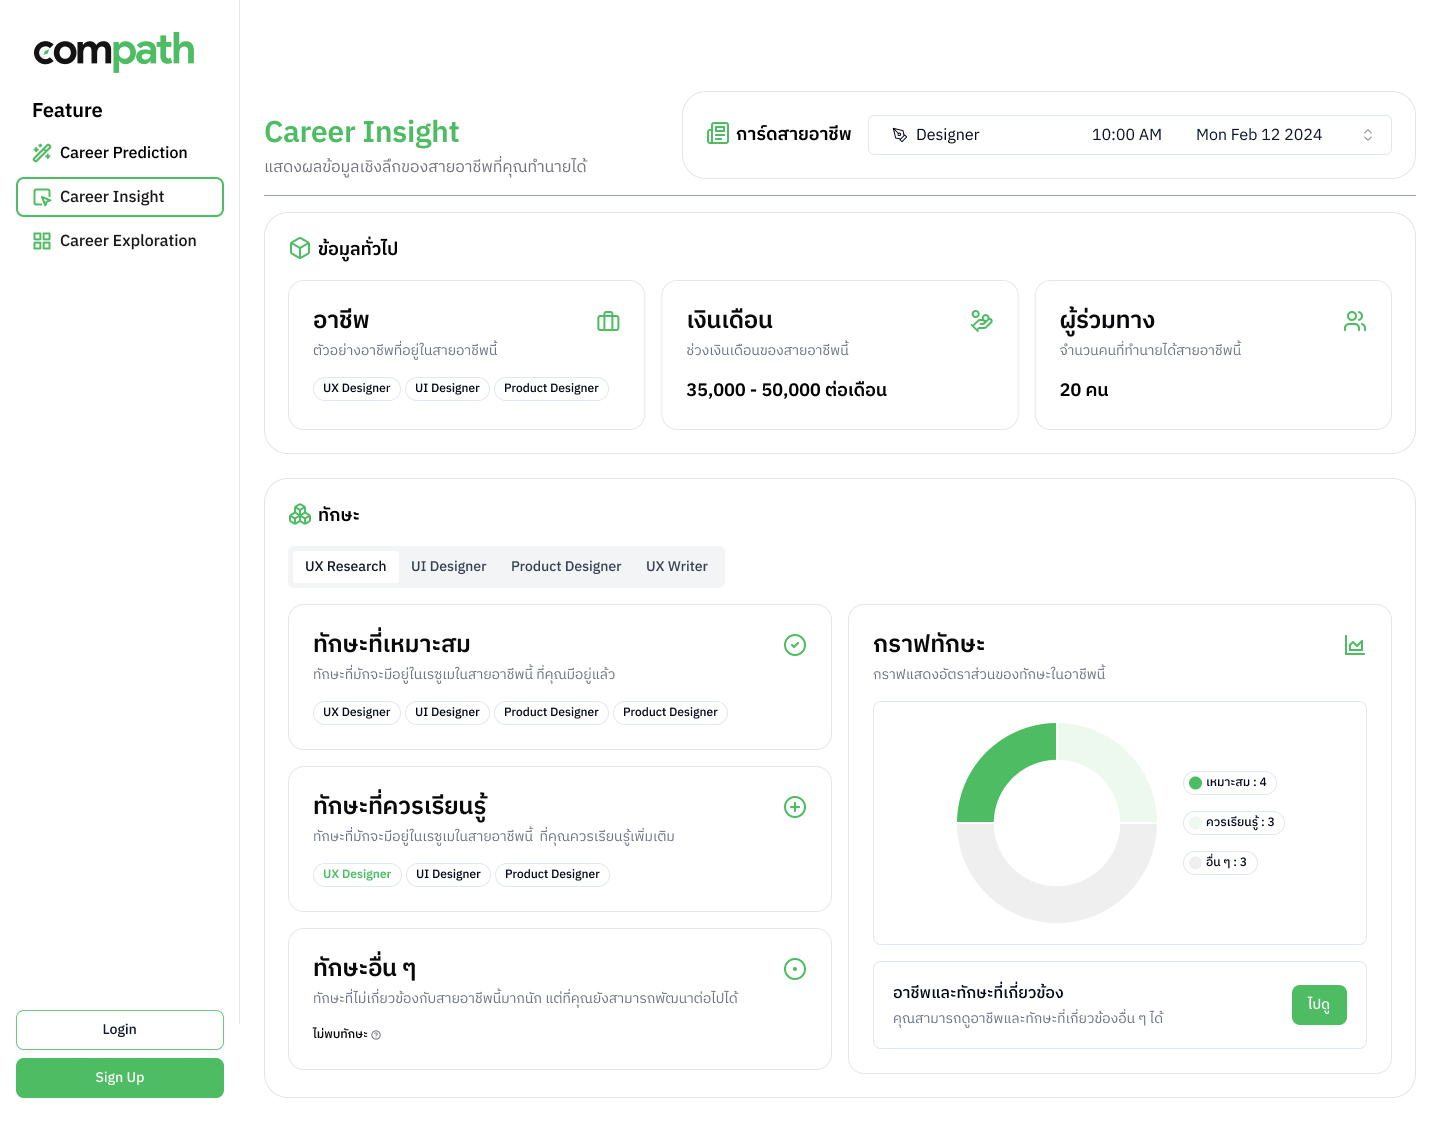
\includegraphics[width=12cm]{./figure/UI-picture/CI.png}}
    \caption{รูปแสดงการออกแบบหน้าข้อมูลเชิงลึกของสายอาชีพที่ทำนายได้}\label{fig:CI.png}
\end{figure}
\begin{figure}[H]\centering
    \fbox{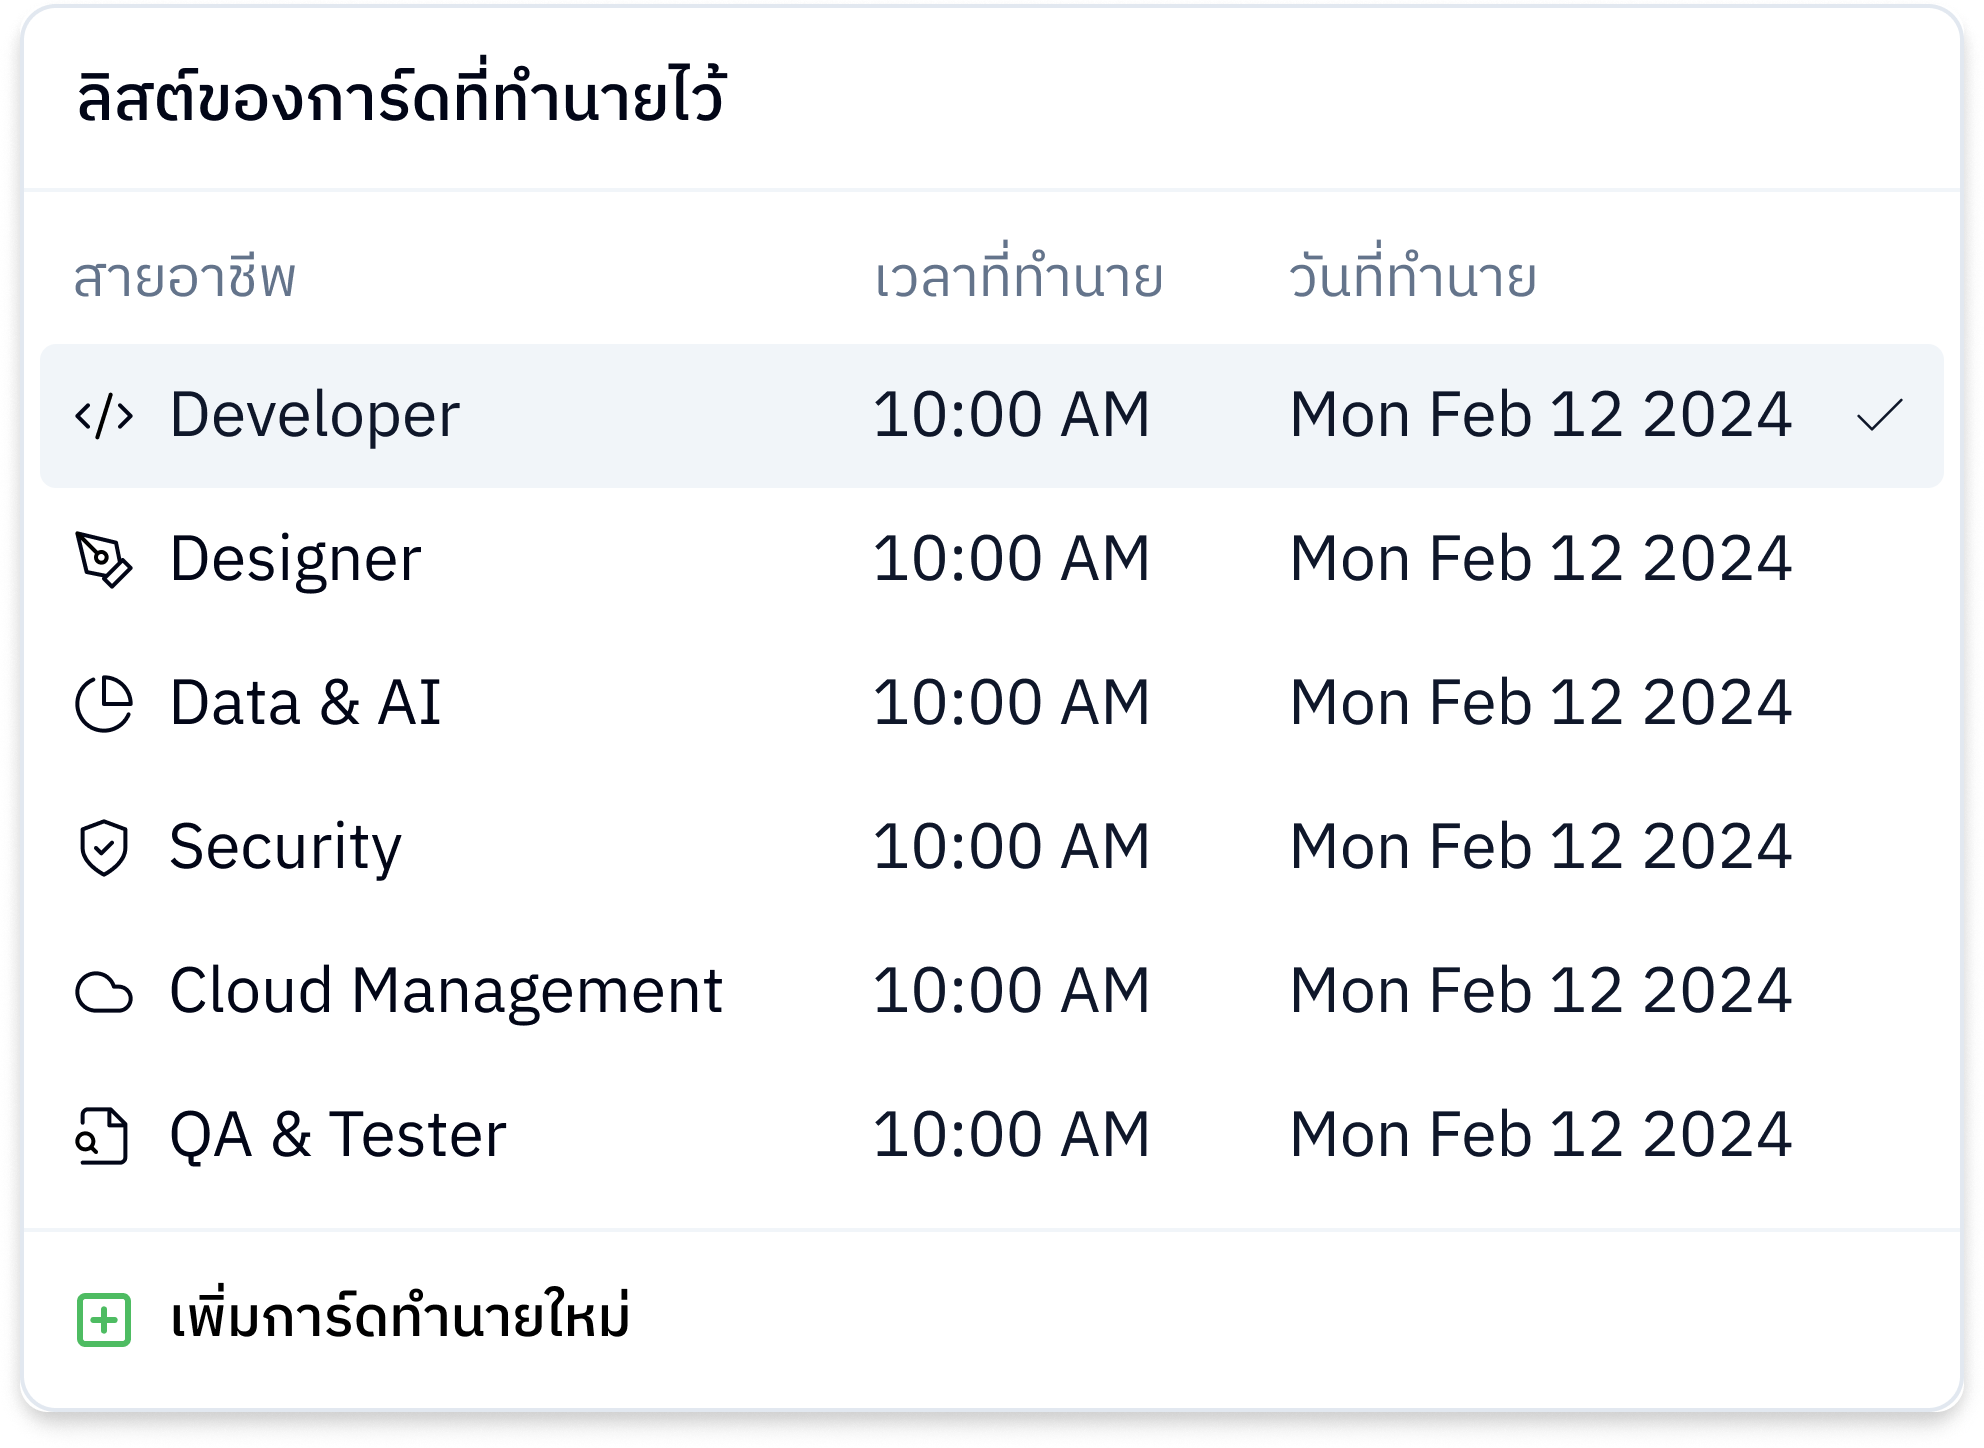
\includegraphics[width=8cm]{./figure/UI-picture/CI-dropdown.png}}
    \caption{รูปแสดงการออกแบบหน้าเมนูเลือกการ์ดที่ถูกทำนาย}\label{fig:CI-dropdown.png}
\end{figure}

\subsection{Career Exploration (สายใยอาชีพ)}
คือหน้าสำหรับดูทักษะที่ควรเรียนรู้ของอาชีพที่สนใจและข้อมูลของอาชีพอื่น ๆ ที่ใกล้เคียง ดังรูป \ref{fig:CE.png} ดังนี้
\begin{figure}[H]\centering
    \fbox{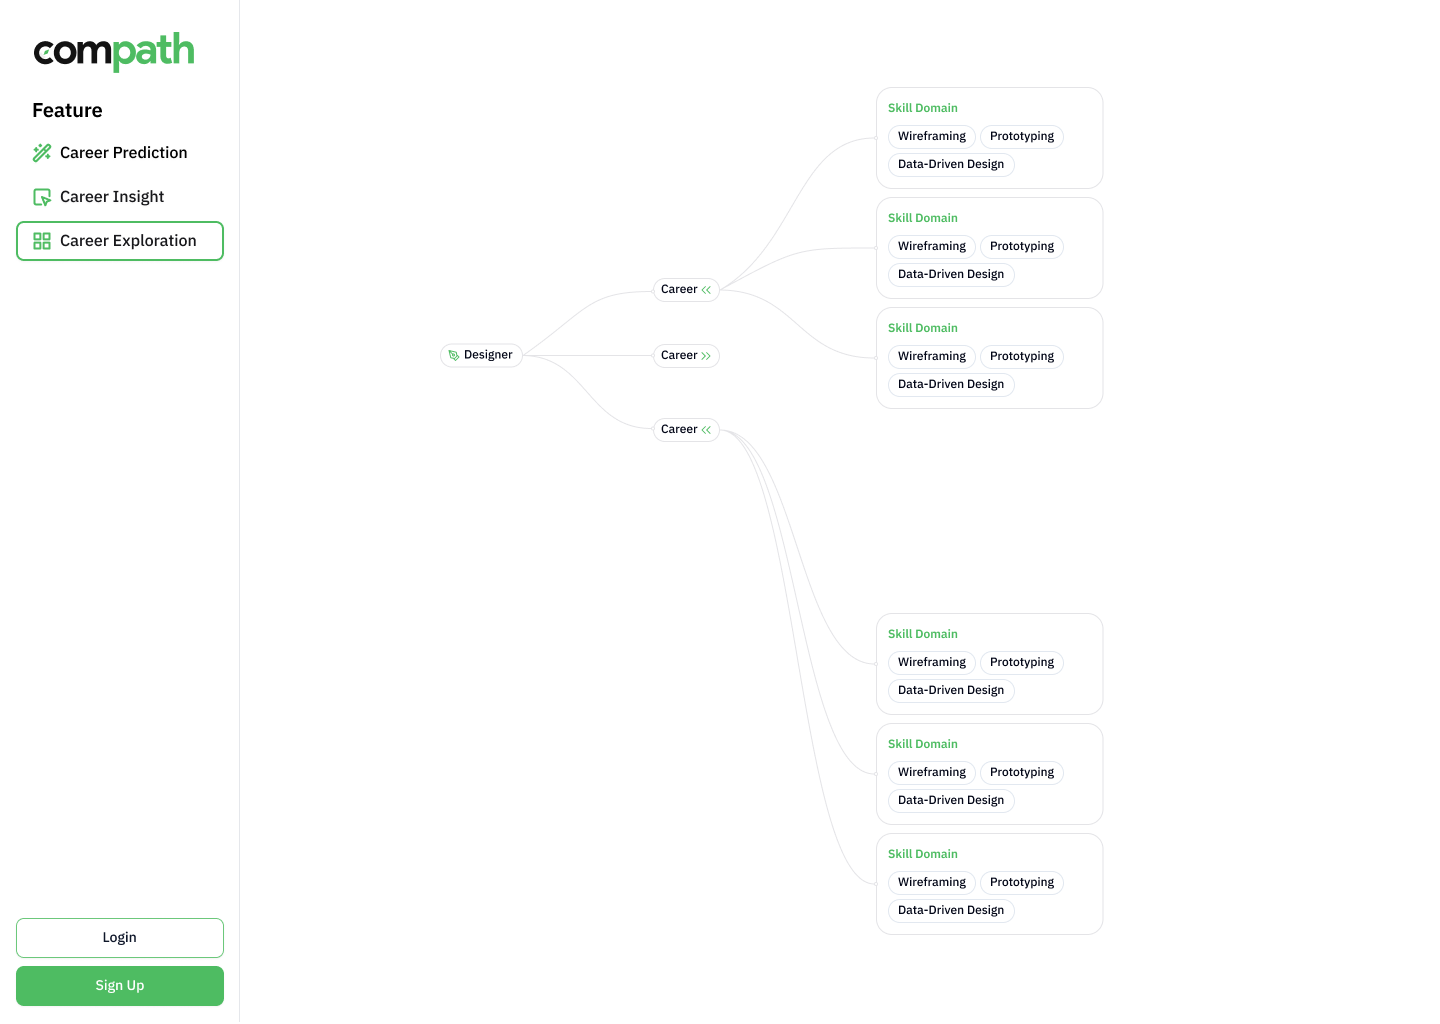
\includegraphics[width=12cm]{./figure/UI-picture/CE.png}}
    \caption{รูปแสดงการออกแบบหน้าสายใยอาชีพ}\label{fig:CE.png}
\end{figure}
%%%%%%%%%%%%%%%%%%%%%%%%%%%%%%%%%%%%%%%%%%%%%%%%%%%%%%%%%%%%%
% Data Modeling Section
%%%%%%%%%%%%%%%%%%%%%%%%%%%%%%%%%%%%%%%%%%%%%%%%%%%%%%%%%%%%%

\section{ขั้นตอนการพัฒนาโมเดล}
\subsection{กำหนดวัตถุประสงค์ และคัดเลือกโมเดลสำหรับการทดลอง}
เพื่อสร้างโมเดลที่ตอบโจทย์กับวัตถุประสงค์ของคณะผู้จัดทำ ซึ่งคือการจำแนกประเภทของเรซูเมให้เหมาะสมกับสายอาชีพ ทางเราสังเกตุเห็นว่า การใช้งานโมเดลในหมวดของการเรียนรู้ของเครื่อง หรือ machine learning นั้น มีโมเดลที่เหมาะสมมากที่สุด ประกอบด้วย
\begin{itemize}
    \item Multinomial Navie Bayes
    \item Gaussian Navie Bayes
    \item K-Neighbors
    \item K-Neighbors with with One vs Rest
    \item Support Vector Machine (SVM)
    \item Logistic Regression
\end{itemize}

อย่างไรก็ตาม ทางคณะผู้จัดทำต้องการจะทดสอบความเป็นไปได้ทางทฤษฎีและค้นหาความเป็นไปได้ใหม่ ๆ หากสามารถทำได้ อาจจะทำให้ได้รับผลลัพธ์ที่ดียิ่งกว่าสิ่งที่คาดไว้ \textbf{จึงได้คิดนำโมเดลประเภทการเรียนรู้เชิงลึก หรือ deep learning มาใช้งานด้วย
ซึ่งคือโมเดล Bidirectional LSTM (Bi-LSTM)} ซึ่งเป็นโมเดลที่สามารถจับความสัมพันธ์ระหว่างลำดับข้อความได้ ซึ่งอาจเหมาะกับข้อมูลภายในเรซูเม อีกทั้งทรัพยากรที่ใช้ยังอยู่ในขอบเขตที่รับไหว โดยทางคณะผู้จัดทำคาดหวังเป็นอย่างมากว่าโมเดล Bi-LSTM จะสามารถสร้างโมเดลที่มีประสิทธิภาพที่ดีตามที่คาดไว้

\subsection{การรวบรวมข้อมูล (Get Data)}
\label{subsec:Data Collecting}
ทางคณะผู้จัดทำได้เลือกนำชุดข้อมูล Updated Resume Dataset \cite{dataset} จาก Kaggle ซึ่งเป็นชุดข้อมูล
ที่ประกอบไปด้วยอาชีพทั้งหมด 25 หมวด และรายละเอียดภายในเรซูเมของแต่ละอันที่จะแตกต่างกันไปในแต่ละอัน ซึ่งมีเรซูเม
ทั้งหมด 962 เล่ม ซึ่งเป็นภาษาอังกฤษทั้งหมด
\begin{figure}[H]\centering
    \setlength{\fboxrule}{0.2mm} % can define this in the preamble
    \setlength{\fboxsep}{0.5cm}
    \fbox{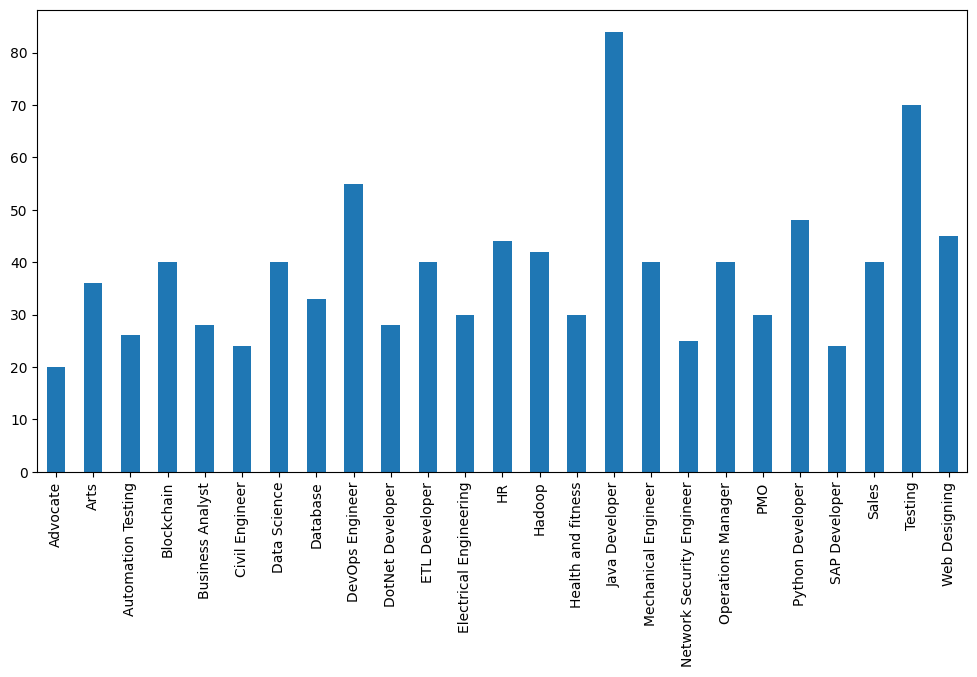
\includegraphics[width=10cm]{./figure/figure_datasetCategory.png}}
    \caption{จำนวนของเรซูเมในแต่ละหมวดอาชีพ}\label{fig:datasetCategory}
\end{figure}
ภายในชุดข้อมูล ในแต่ละแถวจะแสดงถึงข้อมูลภายในเรซูเมนั้น และจะประกอบไปด้วย 2 หลัก ดังต่อไปนี้
\begin{enumerate}
    \item \textbf{Category} : หมวดอาชีพของเรซูเม
    \item \textbf{Resume} : รายละเอียดของเรซูเมที่ประกอบไปด้วย ประวัติการศึกษา, ทักษะ, ประสบการณ์การทำงาน หรือโปรเจค
\end{enumerate}
\begin{figure}[H]\centering
    \setlength{\fboxrule}{0.2mm} % can define this in the preamble
    \setlength{\fboxsep}{0.5cm}
    \fbox{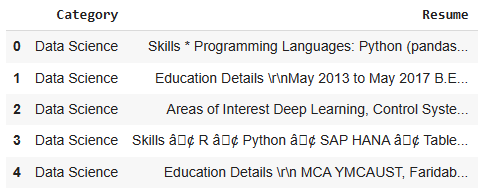
\includegraphics[width=10cm]{./figure/figure_datasetData.png}}
    \caption{ตัวอย่างชุดข้อมูลที่รวบรวมมา}\label{fig:datasetData}
\end{figure}
\par ซึ่งทางคณะผู้จัดทำ จำเป็นต้องทำการเตรียมข้อมูลที่เหมาะสมเพื่อให้โมเดลมีประสิทธิภาพ

\subsection{การเตรียมข้อมูล (Clean, Prepare and Manipulate Data)}
\label{subsec:Data Preparation}
หลังจากที่ทางคณะผู้จัดทำได้ทำการสำรวจชุดข้อมูล ทำให้พบว่ารายละเอียดของเรซูเมยังไม่สามารถนำไปใช้ได้ทันที
เนื่องจากข้อมูลเรซูเม ได้มีตัวอักษรพิเศษรวมอยู่เป็นจำนวนมาก เช่น \^a, €, ¢, \textbackslash r, \textbackslash n
รวมไปถึงมีการใส่ลิงก์ภายนอกอีกด้วย ทางคณะผู้จัดทำจึงจำเป็นที่จะต้องทำให้ตัวหนังสือภายในเรซูเม เป็นเพียงตัวอักษรปกติเท่านั้น
\par เนื่องจากทางคณะผู้จัดทำเล็งเห็นกลุ่มเป้าหมายเป็นนักศึกษาวิศวกรรมคอมพิวเตอร์ มจธ. จึงจำเป็นที่ต้องเลือกเฉพาะข้อมูลที่เป็น
Software Engineer, Data \& AI, Designer, Network Security, Cloud Management, QA \& Tester รวมทั้งหมด 6 สายอาชีพ
ซึ่งคณะผู้จัดจึงต้องลบบางหมวดอาชีพ และทำการรวมบางอาชีพเข้าด้วยกัน โดยพิจารณาจากรายละเอียดของแต่ละสายอาชีพ
ซึ่งในปัจจุบันจะเหลือเรซูเมเพียง 698 เล่มเท่านั้น

\begin{table}[H]
    \caption{ตารางแสดงการจัดหมวดหมู่สายอาชีพใหม่}
    \label{tab:grouping_data}
    \begin{tabularx}{\textwidth}{|l|X|} \hline
        สายอาชีพใหม่        & ประกอบด้วย                                                                                                   \\ \hline
        Software Engineer & Web Designing, Java Developer, SAP Developer, Python Developer, Blockchain, ETL Developer, DotNet Developer \\\hline
        Data \& AI        & Business Analyst,Database,Data Science, Hadoop                                                              \\\hline
        Designer          & Design, *UX/UI Designer, *UX/UI Researcher                                                                  \\\hline
        Network Security  & Network Security Engineer                                                                                   \\\hline
        Cloud Management  & Operations Manager, DevOps Engineer, PMO                                                                    \\\hline
        QA \& Tester      & Testing, Automation Testing, *Software Tester, *Quality Assurance                                           \\\hline
        \multicolumn{2}{l}{หมายเหตุ : * เป็นข้อมูลที่ทางผู้จัดทำหาเพิ่มเติมจาก \href{https://th.jobsdb.com/}{JobDB}}                                 \\ \hline\hline
    \end{tabularx}
\end{table}

และคณะผู้จัดทำได้ใช้อัลกอริทึมในการคัดแยกคำด้วย Term Frequency Inverse Document Frequency (TF-IDF) โดยคณะผู้จัดทำคาดหวังว่า
อัลกอริทึมนี้จะสามารถจับคำสำคัญของแต่ละสายอาชีพได้

\subsection{การเทรนโมเดล (Train Model)}
หลังจากที่ทางคณะผู้จัดทำได้ทำการเตรียมข้อมูลสำเร็จแล้ว คณะผู้จัดทำก็ได้ทำโมเดลขึ้นมาทั้งหมด 7 โมเดล เพื่อเปรียบเทียบ
ซึ่งเป็นโมเดลสำหรับการจัดหมวดหมู่แยกประเภท โดยจะบอกเล่าในส่วนของโมเดลประเภท machine learning ก่อน ดังตารางต่อไปนี้
\begin{table}[H]
    \begin{tabularx}{\textwidth}{|l|l|X|X|} \hline
        \multicolumn{2}{|c|}{โมเดล}                                   & พารามิเตอร์                       & หมายเหตุ                                                       \\ \hline
        \multirow{6}{*}{Navie Bayes}                                 & \multirow{4}{*}{Multinomial}    & alpha = 1.0              &                                    \\ \cline{3-4}
                                                                     &                                 & force\_alpha = True      &                                    \\ \cline{3-4}
                                                                     &                                 & fit\_prior = True        &                                    \\ \cline{3-4}
                                                                     &                                 & class\_prior = None      &                                    \\ \cline{2-4}
                                                                     & \multirow{2}{*}{Gaussian}       & priors = None            &                                    \\ \cline{3-4}
                                                                     &                                 & var\_smoothing = 1e-9    &                                    \\ \hline
        \multirow{7}{*}{K-Neighbors}                                 & \multirow{6}{*}{K-Neighbors*}   & algorithm = brute\_force &                                    \\ \cline{3-4}
                                                                     &                                 & leaf\_size = 30          &                                    \\ \cline{3-4}
                                                                     &                                 & metric = minkowski       &                                    \\ \cline{3-4}
                                                                     &                                 & n\_neighbors = 5         &                                    \\ \cline{3-4}
                                                                     &                                 & p = 2                    & คำนวณด้วยสูตร euclidean               \\ \cline{3-4}
                                                                     &                                 & weight = distance        &                                    \\  \cline{2-4}
                                                                     & One Vs Rest                     & K-Neighbors*             & นำโมเดล K-Neighbors ก่อนหน้ามาใช้งานต่อ \\ \hline
        \multicolumn{2}{|l|}{\multirow{2}{*}{Support Vector Machine}} & kernel = sigmoid                &                                                               \\ \cline{3-4}
        \multicolumn{2}{|l|}{}                                        & decision\_function\_shape = ovr &                                                               \\ \hline
        \multicolumn{2}{|l|}{\multirow{3}{*}{Logistic Regression}}    & C = 5e1                         &                                                               \\ \cline{3-4}
        \multicolumn{2}{|l|}{}                                        & solver = lbfgs                  &                                                               \\ \cline{3-4}
        \multicolumn{2}{|l|}{}                                        & multi\_class = multinomial      &                                                               \\ \hline
    \end{tabularx}
\end{table}

โดยที่ทั้ง 6 โมเดลจะใช้คอลัมน์ Resume จากชุดข้อมูลมาเป็นข้อมูลนำเข้า โดยจะต้องผ่าน\hyperref[subsec:Data Preparation]{การเตรียมข้อมูล}ก่อน ซึ่งจะมีลักษณะเป็น
Term Frequency Inverse Document Frequency (TF-IDF) ในทุกโมเดล

ในส่วนของ ฺBi-LSTM เราได้วางโครงสร้างและขั้นตอนการจัดการข้อมูลก่อนเข้าสู่การเทรนโมเดลเอาไว้ ดังนี้
\begin{itemize}
    \item นำข้อความภายในเรซูเม (Resume) มาผ่านการทำโทเคน (Tokenization) เพื่อแปลงจากอักษรแต่ละตัว ให้กลายเป็นชุดตัวเลขเฉพาะแบบดัชนี (index) เรียงกันเป็นลำดับแทน
    \item นำข้อมูลนำเข้า มาผ่านการเติมค่าว่างให้เต็ม (padding) เพื่อให้มีขนาดของลำดับในขั้นตอนก่อนหน้า มีขนาดเท่ากันเป็นจตุรัส จึงจะนำไปใช้งานและเทรนโมเดลได้
    \item ภายในกระบวนการของโมเดล (Embedding Layer) ข้อมูลอักษรที่กลายเป็นชุดตัวเลข จะถูกนำไปแปลงจากตัวเลขเฉพาะแบบดัชนี ให้กลายเป็นพิกัดเว็กเตอร์แทน
    \item กระบวนการต่อมา (Bi-LSTM Layer) เลเยอร์ของ Bi-LSTM จะทำการเทียบพิกัดและหาความสัมพันธ์ของแต่ละอักษรกับคลาสที่เราวางเอาไว้ โดยใช้แนวคิดของ \hyperref[subsec:lstm]{gate และ state ของ LSTM} ซึ่งจะได้รับผลลัพธ์ออกมาเป็นเวกเตอร์ที่เข้าใกล้กับลักษณะของแต่ละคลาส
    \item ในท้ายที่สุด ณ Output Layer พิกัดจากผลลัพธ์ก่อนหน้าจะถูกนำมาแปลงให้กลายเป็นความน่าจะเป็นที่มีค่าระหว่าง 0 ถึง 1 ด้วยวิธี softmax
    \item คลาสที่มีความน่าจะเป็นสูงสุด จะถูกมองเป็นคำตอบของการแยกประเภทในครั้งนี้
\end{itemize}
ในส่วนของพารามิเตอร์สำหรับแต่ละขั้นตอนของ Bi-LSTM เราได้ตั้งค่าไว้ ดังนี้
\begin{itemize}
    \item Embedding Layer ซึ่งมีขนาดมิติของเว็กเตอร์ได้สูงสุด 100*100
    \item Bi-LSTM ขนาด 128 units พร้อม dropout rate 40\% เพื่อป้องกันการ overfit
    \item Bi-LSTM ขนาด 64 units พร้อม dropout rate 40\% เพื่อป้องกันการ overfit
    \item Dense Layer as Output ขนาด 6 (เท่ากับจำนวนคลาสผลลัพธ์ของเรา) และมี softmax เป็น activation function
\end{itemize}


\par และคณะผู้จัดทำก็จะทำการใส่ข้อมูลที่เตรียมเอาไว้เพื่อทำการเทรนโมเดลทั้งหมด โดยที่โมเดลทุกตัวจะทำหน้าที่เดียวกัน คือทำการทำนายว่าข้อมูลเรซูเมที่ใส่เข้าไป
เป็นอาชีพใดจากทั้งหมด 6 อาชีพ (Software Engineer, Data \& AI, Designer, Network Security, Cloud Management, QA \& Tester)
ดัง\textbf{ตารางที่ \ref{tab:grouping_data}} ซึ่งสามารถแสดงผลออกมาเป็นอาชีพที่คาดว่ามีลักษณะใกล้เคียงที่สุด

\subsection{การทดสอบข้อมูล (Test Data)}
หลังจากที่คณะผู้จัดทำได้เทรนโมเดลจนสำเร็จแล้ว ก็ได้ลองนำเรซูเมของคณะผู้จัดทำมาลองกับโมเดล ซึ่งผลลัพธ์ที่ได้ก็ค่อนข้างน่าพอใจ
คาดว่าเนื่องจากมีสายอาชีพที่ต้องทำนายค่อนข้างน้อย ทำให้มีโอกาสที่จะทำนายได้ถูกต้องค่อนข้างสูง

\subsection{การพัฒนาโมเดล (Improvement)}
ทางคณะผู้จัดทำคาดหวังว่าจะพัฒนาโมเดลได้ด้วยการหาชุดข้อมูลสำหรับการเทรนมากขึ้นกว่านี้ ทดลองเพิ่มจำนวน Epoch สำหรับการเทรน
Long Short Term Memory (LSTM) ที่มากกว่านี้ การจัดเตรียมข้อมูลที่อาจสนับสนุนการเรียนรู่ของโมเดลมากกว่าเดิม และคาดหวังว่าในอนาคตจะมีสายอาชีพที่ทำการทำนายเพิ่มมากขึ้นกว่าในปัจจุบันนี้

%%%%%%%%%%%%%%%%%%%%%%%%%%%%%%%%%%%%%%%%%%%%%%%%%%%%%%%%%%%%%
% Evaluation Method Section
%%%%%%%%%%%%%%%%%%%%%%%%%%%%%%%%%%%%%%%%%%%%%%%%%%%%%%%%%%%%%

\section{วิธีการวัดผล}
ในส่วนของการวัดผล เนื่องจากโครงงานของเราประกอบด้วย 2 ส่วนซึ่งแยกกันได้ชัดเจน คือ ประสบการณ์การใช้งานเว็บแอปพลิเคชันที่ตอบโจทย์ปัญหาที่เราคาดการณ์ว่าจะสามารถแก้ได้
และโมเดลปัญญาประดิษฐ์ที่สามารถมอบคำตอบที่พึงพอใจแก่ผู้ใช้งานได้ตามที่คาดหวัง ดังนั้น เราจึงแบ่งวิธีการวัดผลออกเป็น 2 ส่วนเช่นกัน ดังนี้

\begin{enumerate}
    \item การวัดผลเว็บแอปพลิเคชัน: เราคาดการณ์จะวัดผลด้วยการทดสอบกับผู้ใช้งานกลุ่มตัวอย่าง (Usability Test) จำนวน 5 คน จากนั้นจึงเก็บความเห็นและคะแนนความพึงพอใจจากผู้ทดสอบ
          โดยเราคาดหวังว่าจะได้ผลตอบรับในเชิงบวกและได้รับคะแนนมากกว่าร้อยละ 70 จึงจะถือว่าสำเร็จ
    \item การวัดผลโมเดล: เนื่องจากการเทรนโมเดลของพวกเรา เป็นการเทรนที่ต้องทำให้เกิดการ overfit ดังนั้นจึงไม่สามารถใช้เกณฑ์ความแม่นยำปกติในการสรุปผลได้
          เราจึงออกแบบวิธีการวัดผลโดยการทดสอบกับผู้ใช้เช่นเดียวกับเว็บแอปพลิเคชัน อย่างไรก็ตาม การวัดความพึงพอใจกับโมเดลทำนายผลเช่นนี้
          ผู้ทดสอบอาจเกิดความลำเอียงกับคำตอบในใจได้ เราจึงออกแบบเงื่อนไขการวัดผลเพื่อความรัดกุมและมีประสิทธิภาพ ดังนี้
          \begin{itemize}
              \item เราจะทดสอบกับผู้ใช้ 25 คน
              \item ผู้ทดสอบจะต้องบอกคำตอบที่คาดหวังในใจของตนเองก่อนล่วงหน้าที่จะได้รับคำตอบจากโมเดล
              \item ผู้ทดสอบให้อนุญาติเก็บข้อมูลอินพุตของเรซูเมตนเอง
              \item ให้บุคคลภายนอกจำนวน 2-3 คน อ่านข้อมูลอินพุตผู้ทดสอบ และทดลองให้คำทำนายในมุมของบุคคลภายนอกด้วย
              \item หากผู้ทดสอบพึงพอใจกับคำตอบของโมเดล ถือว่าการทดลองรอบนั้นสำเร็จผลทันที
              \item หากผู้ทดสอบยังไม่พอใจกับคำตอบของโมเดล และความเห็นจากบุคคลภายนอกเห็นพ้องด้วย ถือว่าการทดลองรอบนั้นไม่สำเร็จ
              \item หากผู้ทดสอบยังไม่พอใจกับคำตอบของโมเดล แต่ความเห็นจากบุคคลภายนอกตรงกันข้าม ถือว่าการทดลองรอบนั้นเป็นโมฆะ
              \item เราคาดหวังว่าโมเดลจะสร้างความพอใจกับผู้ใช้ได้มากกว่าร้อยละ 70 จากทั้งหมด จึงจะถือว่าประสบความสำเร็จ
          \end{itemize}
\end{enumerate}

% \emph{หัวข้อต่าง ๆ ในแต่ละบทเป็นเพียงตัวอย่างเท่านั้น หัวข้อที่จะใส่ในแต่ละบทขึ้นอยู่กับโปรเจคของนักศึกษาและอาจารย์ที่ปรึกษา}


% ตัวอย่างการใส่อ้างอิงที่มา -> \cite{hypersense} ถ้าต้องการใส่แหล่งอ้างอิงมากกว่า 1 ให้ทำดังนี้ -> \cite{hypersense,bworld}
% Explain the design (how you plan to implement your work) of your project. Adjust the section titles below to suit the types of your work. Detailed physical design like circuits and source codes should be placed in the appendix.

% \section{ข้อกำหนดและความต้องการของระบบ}

% \section{สถาปัตยกรรมระบบ}

% \begin{table}[!h]
%     % \centering
%     \caption{test table x1}\label{tbl:symbols}
%     \begin{tabular}{@{}p{0.07\textwidth}|p{0.7\textwidth}p{0.1\textwidth}}\hline
%         \multicolumn{2}{l}{\textbf{SYMBOL}} & \textbf{UNIT}                         \\ \hline
%         $\alpha$                            & Test variable\hfill     & m$^2$       \\
%         $\lambda$                           & Interarrival rate\hfill & jobs/second \\
%         $\mu$                               & Service rate\hfill      & jobs/second \\ \hline
%     \end{tabular}
%     %\begin{tabular}{c|c} \hline
%     % $\alpha$ & $\beta$ \\ \hline
%     % $\delta$ & $\mu$ \\ \hline
%     %\end{tabular}
% \end{table}



% \section{Hardware Module 1}
% \subsection{Component 1}
% \subsection{Logical Circuit Diagram}

% \section{Hardware Module 2}
% \subsection{Component 1}
% \subsection{Component 2}

% \section{Path Finding Algorithm}

% \section{Database Design}

% \section{UML Design}

% \section{GUI Design}

% \section{การออกแบบการทดลอง}
% \subsection{ตัวชี้วัดและปัจจัยที่ศึกษา}
% \subsection{รูปแบบการเก็บข้อมูล}